%!TEX program = lualatex
%----------------------------------------------------------------------------------------
%	PACKAGES AND THEMES
%----------------------------------------------------------------------------------------
\documentclass[aspectratio=169,xcolor=dvipsnames, t]{beamer}
\usepackage{fontspec} % Allows using custom font. MUST be before loading the theme!
\usetheme{SimplePlusAIC}
\usepackage{hyperref}
\usepackage{graphicx} % Allows including images
\usepackage{booktabs} % Allows the use of \toprule, \midrule and  \bottomrule in tables
\usepackage{svg} %allows using svg figures
\usepackage{tikz}
\usepackage{makecell}
\usepackage{wrapfig}
\usepackage{braket}
%\usepackage{appendixnumberbeamer}
% ADD YOUR PACKAGES BELOW

%----------------------------------------------------------------------------------------
%	TITLE PAGE CONFIGURATION
%----------------------------------------------------------------------------------------

\title[short title]{AKLT-States as ZX-Diagrams} % The short title appears at the bottom of every slide, the full title is only on the title page
\subtitle{Diagrammatic Reasoning for Quantum States}

\author[Surname]{East, R. D., van de Wetering, J., Chancellor, N., \& Grushin, A. G. (2022)\\ PRX quantum, 3(1), 010302.}
\institute[]{Presented by Yan Mong Chan}
% Your institution as it will appear on the bottom of every slide, maybe shorthand to save space


\date{\today} % Date, can be changed to a custom date
%----------------------------------------------------------------------------------------
%	PRESENTATION SLIDES
%----------------------------------------------------------------------------------------

\begin{document}

\maketitlepage

\begin{frame}[t]{Overview}
    % Throughout your presentation, if you choose to use \section{} and \subsection{} commands, these will automatically be printed on this slide as an overview of your presentation
    \tableofcontents
\end{frame}

%------------------------------------------------
\makesection{AKLT Model}
\begin{frame}{AKLT Model}
    \begin{itemize}
        \item Spin-1 Affleck-Kennedy-Lieb-Tasaki (AKLT) model with $N$ sites
        \begin{align}
            H^{S=1}_\text{AKLT} &=\frac{1}{24}\sum_{j=1}^{N-1}(\mathbf S_j + \mathbf S_{j+1})^2 \left((\mathbf S_j + \mathbf S_{j+1})^2-2\right)\\ &=\frac{1}{2} \sum_{j=1}^{N-1} \left[\mathbf S_j \cdot \mathbf S_{j+1} + \frac{1}{3} (\mathbf S_{j} \cdot \mathbf S_{j+1})^2 +\frac{2}{3}\right] \nonumber
        \end{align}
        \item $\mathbf S_{i}$ are 3x3 spin-1 operators; $\mathcal H =\mathbb C_2^{\otimes N}$ 
    \end{itemize}
\end{frame}

\begin{frame}{Why interesting?}
    \begin{itemize}
        \item Historically, it was believed that the GS of 1D spin chains of any spins are gapless
        \item An example that verifies the Haldane conjecture: integer spin antiferromagnetic Heisenberg chains has gapped GS 
        \item Lots of surprising physics: Hidden string order, etc. 
    \end{itemize}
\end{frame}

%\begin{frame}{Why interesting?}
%    \begin{block}{Frustration Free}
%        
%    \end{block}
%    \begin{itemize}
%        \item It is gapped (Any proof?)
%        \item It has exponentially decaying correlation function (Any proof?)
%        \item It is an example that verifies the Haldane conjecture in 1 dimension (What is the Haldane conjecture?)
%    \end{itemize}
%\end{frame}

\begin{frame}{Ground state of Spin-1 AKLT}
    \begin{itemize}
        \item The Hamiltonian is a projector onto adjacent total spin=2 subspace because
        \begin{align*}(\mathbf S_j + \mathbf S_{j+1})^2 \left((\mathbf S_j + \mathbf S_{j+1})^2-2\right)\ket{s_\text{total}^{(j,\,j+1)}=0} = 0\\
        (\mathbf S_j + \mathbf S_{j+1})^2 \left((\mathbf S_j + \mathbf S_{j+1})^2-2\right)\ket{s_\text{total}^{(j,\,j+1)}=1} = 0\\
        \end{align*}
        \item Therefore we have
        $$\braket{s_{total}^{(j,\, j+1)} = 2\,\,|\psi_0} = 0\quad \forall j=1,2,\cdots ,N-1$$
        \item $\ket{\psi_0}$ is the ground state(s) of the Hamiltonian
    \end{itemize}
\end{frame}

\begin{frame}
\begin{itemize}
    \item To solve GS, replace each spin-1 site with two spin-1/2 
    \item We construct the state so that spins on adjacent sites are in singlet configuration.
    $$\frac{1}{\sqrt{2}} \left(\ket{0}_i\ket{1}_{i+1}-\ket{1}_i\ket{0}_{i+1}\right)$$
    \item This construction ensures that the total spin on adjacent sites are zero. 
    
    \item We then do a projection onto the the spin-1 subspace for each lattice site
    $$\ket{\uparrow\uparrow}, \frac{1}{\sqrt{2}}\left(\ket{\uparrow\downarrow}+\ket{\downarrow\uparrow}\right),\ket{\downarrow\downarrow}$$
    \item The ground state wavefunction is unique for close chains and 4-fold degenerate for open-end chains
\end{itemize}
\end{frame}

\begin{frame}{MPS representation}
    \begin{figure}
        \centering
        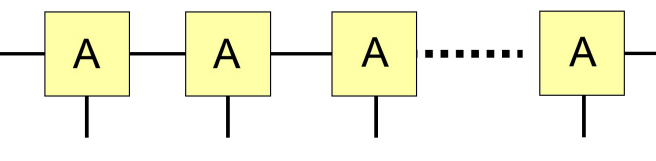
\includegraphics{figures/MPS_AKLT_chain.png}
        \caption{MPS representation of AKLT ground state taken from Wei et. al. (2022) [2201.09307]}
    \end{figure}
\end{frame}


\begin{frame}{Derivation of the MPS representation}
    \begin{itemize}
        \item This derivation is taken from a very useful review by \href{https://www.tmqs.lu/images/haller_bsc.pdf}{Andreas Haller}
        \item Let $\ket{\mathbf a} = \ket{a_1, a_2, \cdots, a_N}$ and $\ket{\mathbf b} = \ket{b_1, b2, \cdots, b_N}$ be the auxiliary spin-1/2 states and $N$ be the number of sites. The general wavefunction takes the form
        $$\ket{\psi} = \sum_{\mathbf a, \mathbf b} c_{\mathbf a\mathbf b} \ket{\mathbf a,\mathbf b}$$
        \item The G.S. adjacent spins are in valence bond, so we have $c_{\mathbf a\mathbf b} = \Sigma_{b_1 a_2}\Sigma_{b_2 a_3}\cdots \Sigma_{b_{N-1} a_{N}}$, where $$\Sigma=\begin{pmatrix}0 & \frac{1}{\sqrt 2}\\-\frac{1}{\sqrt 2} & 0\end{pmatrix}$$
    \end{itemize}
\end{frame}
\begin{frame}
    \begin{itemize}
        \item We the project our subspace onto the spin-1 subspace using the on-site projector
        $$P_i=\sum_{a_i, b_i, \sigma_i} M^{\sigma_i}_{a_ib_i} \ket{\sigma_i}\bra{a_i,b_i}$$
        where $\sigma_i=0,\pm1$, $a_i, b_i = \pm 1/2$, and the matrices $M^\sigma$ takes the form
        $$M^{(1)}=\begin{pmatrix}1 & 0 \\ 0 & 0 \end{pmatrix}\quad M^{(0)}=\begin{pmatrix}0 & \frac{1}{\sqrt 2} \\ \frac{1}{\sqrt 2} & 0 \end{pmatrix}\quad M^{(-1)}=\begin{pmatrix}0 & 0 \\ 0 & 1 \end{pmatrix}$$
        \item Therefore, $\ket{\psi_{0}} \propto P_1 P_2 \cdots P_N \ket{\psi}$, which takes the form
        \begin{align*}
        \ket{\psi_0}&\propto \sum_{\mathbf a, \mathbf b, \boldsymbol \sigma} M^{\sigma_1}_{a_1b_1}\Sigma_{b_1 a_2} M^{\sigma_2}_{a_2 b_2}\Sigma_{b_2 a_3} \cdots \Sigma_{b_{N-1}a_N}M^{\sigma_N}_{a_N b_N} \ket{\boldsymbol{\sigma}}\\
        &= \sum_{\boldsymbol \sigma}A^{\sigma_1}A^{\sigma_2} \cdots A^{\sigma_N} \ket{\boldsymbol \sigma}
        \end{align*}
        where $A^{\sigma_i} = M^{\sigma_i}\Sigma$ and we contract all the $A$s via matrix multiplication
    \end{itemize}
\end{frame}
\begin{frame}
\begin{itemize}
    \item The tensor-trian at each site is given by 
    \begin{align*}
        A^{(+1)} \propto \begin{pmatrix}
            0 & 1 \\
            0 & 0
        \end{pmatrix}\quad A^{(0)} \propto -\frac{1}{\sqrt 2}\begin{pmatrix}
            1 & 0 \\
            0 & -1
        \end{pmatrix} \quad A^{(-1)}\propto \begin{pmatrix}
            0 & 0 \\
            -1 & 0
        \end{pmatrix}
    \end{align*}
    %\item More generally we perform singular-value decomposition (SVD) to obtain the matrix produce state. This is always possible, and the details is outlined in the seminal paper by Oseledets (Tensor-Train Decomposition, SIAM Journal on Scientific Computing 33, 2295-2317 (2011))
    \item Under the convention used by the paper, the MPS matrices are \footnote{MPS matrices are undetermined up to a local change of basis of form $A \mapsto M A M^{-1}$. It is easy to see that the two sets of matrices are related by $\mathcal M^{(n)}=\sigma_x A^{(n)} \sigma_x$}
    \begin{align*}
        \boxed{{\cal M}^{[n]+1}=\sqrt{\frac{2}{3}}\left(\begin{array}{l l}{{0}}&{{0}}\\ {{1}}&{{0}}\end{array}\right)\quad {\cal M}^{[n]0}=\frac{1}{\sqrt{3}}\left(\begin{array}{l l}{{1}}&{{0}}\\ {{0}}&{{-1}}\end{array}\right) \quad {\cal M}^{[n]-1}=\sqrt{\frac{2}{3}}\left(\begin{array}{l l}{{0}}&{{-1}}\\ {{0}}&{{0}}\end{array}\right)}
    \end{align*}
\end{itemize}
\end{frame}

\begin{frame}{Hidden string order}
    \begin{itemize}
        \item The AKLT state has a hidden anti-ferromagnetic order 
        \begin{align*}
            \cdots 1,0,0,0,-1,0,1,0,0,-1\cdots
        \end{align*}
        i.e. successive non-zero spins must be alternating 
        \vspace{.5cm}
        \item In MPS picture, the matrix element of states of form $\ket{\cdots\pm 1,0,0,0,0,\pm 1\cdots}$ is a product of form
        \begin{align*}
            (\cdots) \sigma_{\pm} \sigma_z^n \sigma_{\pm}(\cdots)
        \end{align*}
        \item This is obviously zero because $\{\sigma_\pm,\sigma_z\}=0$ and $\sigma_{\pm}^2=0$
        %\item A string order parameter can used to probe the order
        %\begin{align*}
        %    \Pi_{i,i+r}^\alpha = S_{i}^\alpha e^{i\pi \sum_{j=i+1}^{i+r-1}S^{\alpha}_j} S^{\alpha}_{i+r}
        %\end{align*}
        %where $\alpha=x,y,z$ are the direction of the spins, and $i$ is the length of the site index.
    \end{itemize}
\end{frame}

\begin{frame}{Quantized Berry phase}
    \begin{itemize}
        \item The Berry phase of a \textbf{periodic} 1D AKLT state can be calculated by twisting one of the covalent bonds
        $$\ket{10} - \ket{01}\to \ket{10} - e^{i\theta}\ket{01}$$
        \item The Berry phase is then defined as
        $$\gamma = -i \int_{0}^{2\pi} \frac{\braket{\psi_\theta| \partial_\theta |\psi_\theta}}{\braket{\psi_\theta|\psi_\theta}} d\theta$$
        \item Thermodynamic limit, $\boxed{\gamma = \pi}$ \cite{hatsugai2006quantized}
        \footnote{According to my understand, this phase is quantized (though I can't follow the exact argument), so does it mean that showing $\gamma=\pi$ in thermodynamic limit is the same as showing it for all finite length?}
    \end{itemize}
\end{frame}


%\begin{frame}{Properties of Spin-1 AKLT G.S.}
%    \begin{block}{Frustration Free}
%        $\ket{\psi_0}$ is the G.S. of each term in the Hamiltonian $\implies$  Frustration free
%    \end{block}
%    \begin{block}{\# of degeneracies}
%        G.S. is unique for closed chains, and 4-fold degenerate for open chains
%    \end{block}
%    \begin{block}{Gapped}
%        The groud state is gapped in the sense that $\Delta =\liminf_{n\to \infty}|E^{(n)}_1 - E^{(n)}_0| > 0$
%        where $E^{(n)}_0,E^{(n)}_1$ are the ground state and first-excited state energy of the length-$n$ system, respectively.
%    \end{block}
%\end{frame}


%\begin{frame}{Symmetry protected topological (SPT) phase }
%\begin{itemize}
%    \item The ground state is topologically trivial if it can be smoothly connected connect to a state with no entanglement between local degrees of freedom
%    \item Equivalently (proof needed), 
%\end{itemize}
%\end{frame}


\begin{frame}{G.S. degeneracies of Spin-1 AKLT}
    \begin{itemize}
        \item Replace each spin-1 site with a triplet: $\ket{\uparrow\uparrow}, \frac{1}{\sqrt{2}}\left(\ket{\uparrow\downarrow}+\ket{\downarrow\uparrow}\right),\ket{\downarrow\downarrow}$
        \item For any adjacent site $\mathbf 3\otimes \mathbf3=\mathbf 1 \oplus \mathbf 3 \oplus \mathbf 5$, the combined states lies in $\mathbf 1 \oplus \mathbf 3$ iff there's a valence bond (singlet) between adjacent sites
        \item The G.S. forms valence bond on adjacent sites
        \item If the chain is periodic, only one G.S.
        \item If the chain has open ends, then we have 2 free ends so there are 4 degenerate G.S.
        \item \textit{Question: I have written down the CG decomposition of the two site case and notice something weird that I don't know how to explain}
    \end{itemize}
\end{frame}


\makesection{ZXH Calculus}
\begin{frame}{ZXH Calculus}
\begin{itemize}
    \item Like MPS, a diagrammatic representation of tensors
    \item Equipped with \textit{spiders} with a set of rewriting rules

\end{itemize}
    \begin{figure}
        \centering
        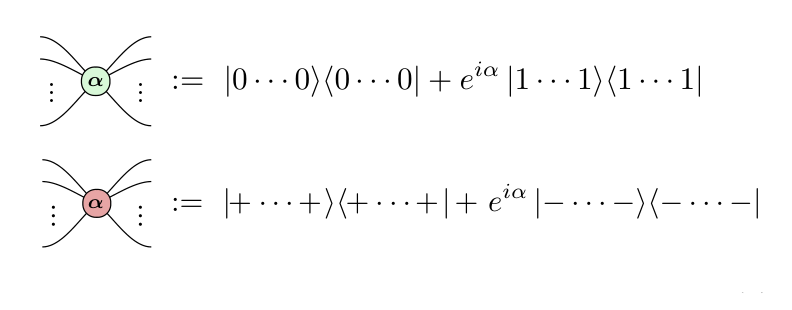
\includegraphics[width=0.8\textwidth]{figures/zx_spiders.png}
    \end{figure}
\end{frame}

\begin{frame}
    \begin{itemize}
        \item There are 3 types of spiders : \textcolor{teal}{Z-spider (light/green)}, \textcolor{red}{X-spider (dark/red)}, and \textcolor{blue}{H-spider (rectangle box)}
        \item Each spider has $n$ inputs, $m$ output, and a phase $\alpha$
    \end{itemize}

    \begin{equation*}
    [Z(\alpha)]^{j_1 j_2 \cdots j_m}_{i_1 i_2 \cdots i_n} = \begin{cases}
        1\quad \quad i_1=i_2=\cdots=j_1=j_2\cdots=j_m = 0\\
        e^{i\alpha} \quad i_1=i_2=\cdots=j_1=j_2\cdots=j_m = 1\\
        0 \quad \text{otherwise}
    \end{cases}
    \end{equation*}
    \begin{equation*}
    [X(\alpha)]^{j_1 j_2 \cdots j_m}_{i_1 i_2 \cdots i_n} = \frac{1}{2^{(n+m)/2}}\begin{cases}
        1+ e^{i\alpha}\quad \left(\oplus_\alpha i_\alpha\right) \oplus \left(\oplus_\beta j_\beta\right)=0\\
        1-e^{i\alpha} \quad \left(\oplus_\alpha i_\alpha\right) \oplus \left(\oplus_\beta j_\beta\right)=1\\
        0 \quad \text{otherwise}
    \end{cases}
    \end{equation*}
    \begin{equation*}
    [H(\alpha)]^{j_1 j_2 \cdots j_m}_{i_1 i_2 \cdots i_n} = \begin{cases}
        a\quad \quad i_1=i_2=\cdots=j_1=j_2\cdots=j_m = 1\\
        1 \quad \text{otherwise}
    \end{cases} \footnote{When $\alpha$ is left unspecified, it is understood that $\alpha=0$ for Z and X, and $\alpha=-1$ for H}
    \end{equation*}
\end{frame}

\begin{frame}
    \begin{itemize}
        \item ZX calculus also comes with a set of rewriting rules 
        \begin{figure}
            \centering 
            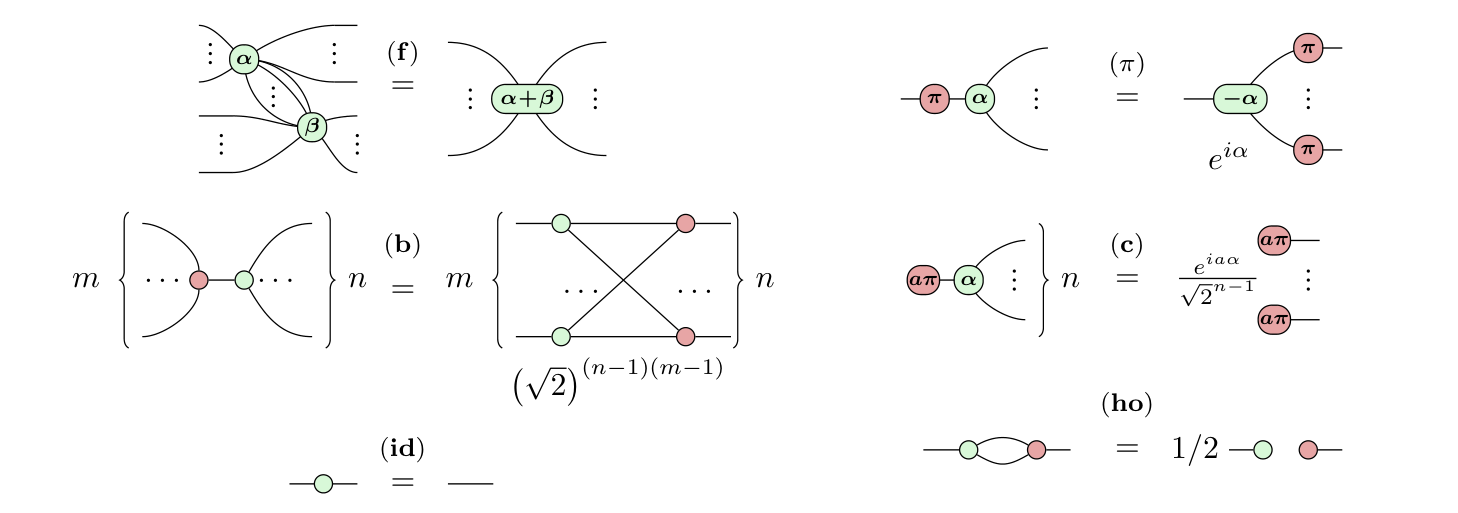
\includegraphics[width=\textwidth]{figures/zx_rewrite_rules_p1.png}
        \end{figure}
        \item and etc. etc.
        \item A comprehensive introduction of these rules can be found in \cite{zx_for_working_qcs}. For reference, I have listed these rules in the appendix of the slides.
    \end{itemize}
\end{frame}

\begin{frame}{Example - States}
% |0>, |1>, |+>, |->
% The bell state etc.
\begin{figure}
    \centering
    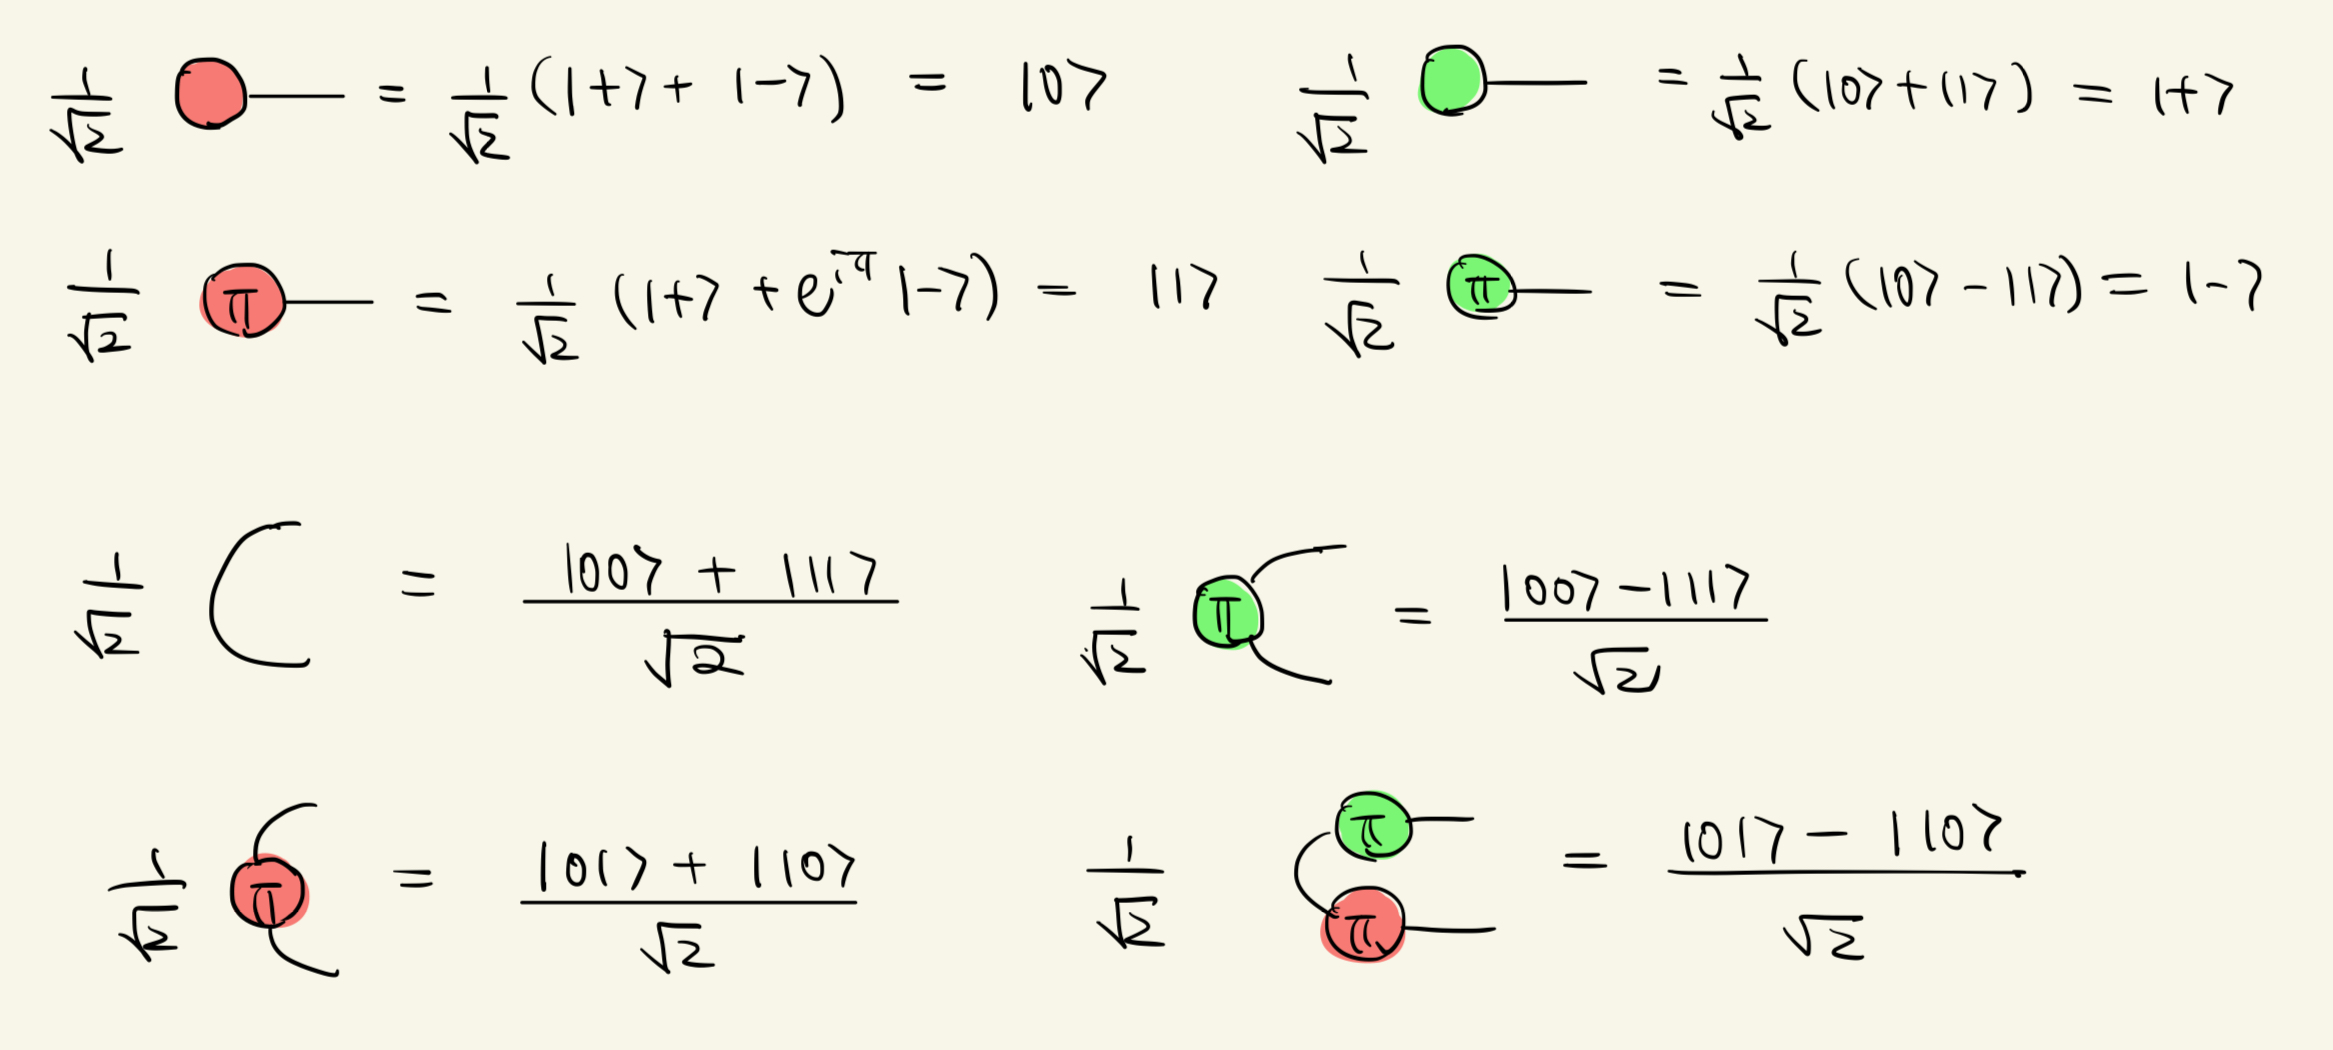
\includegraphics[width=1.\textwidth]{figures/zx_states.PNG}
\end{figure}
\end{frame}

\begin{frame}{Example - Circuit gates}
    % CNOT gate, CX gate, X gate, Z gate, H gate, etc. 
    \begin{figure}
        \centering
        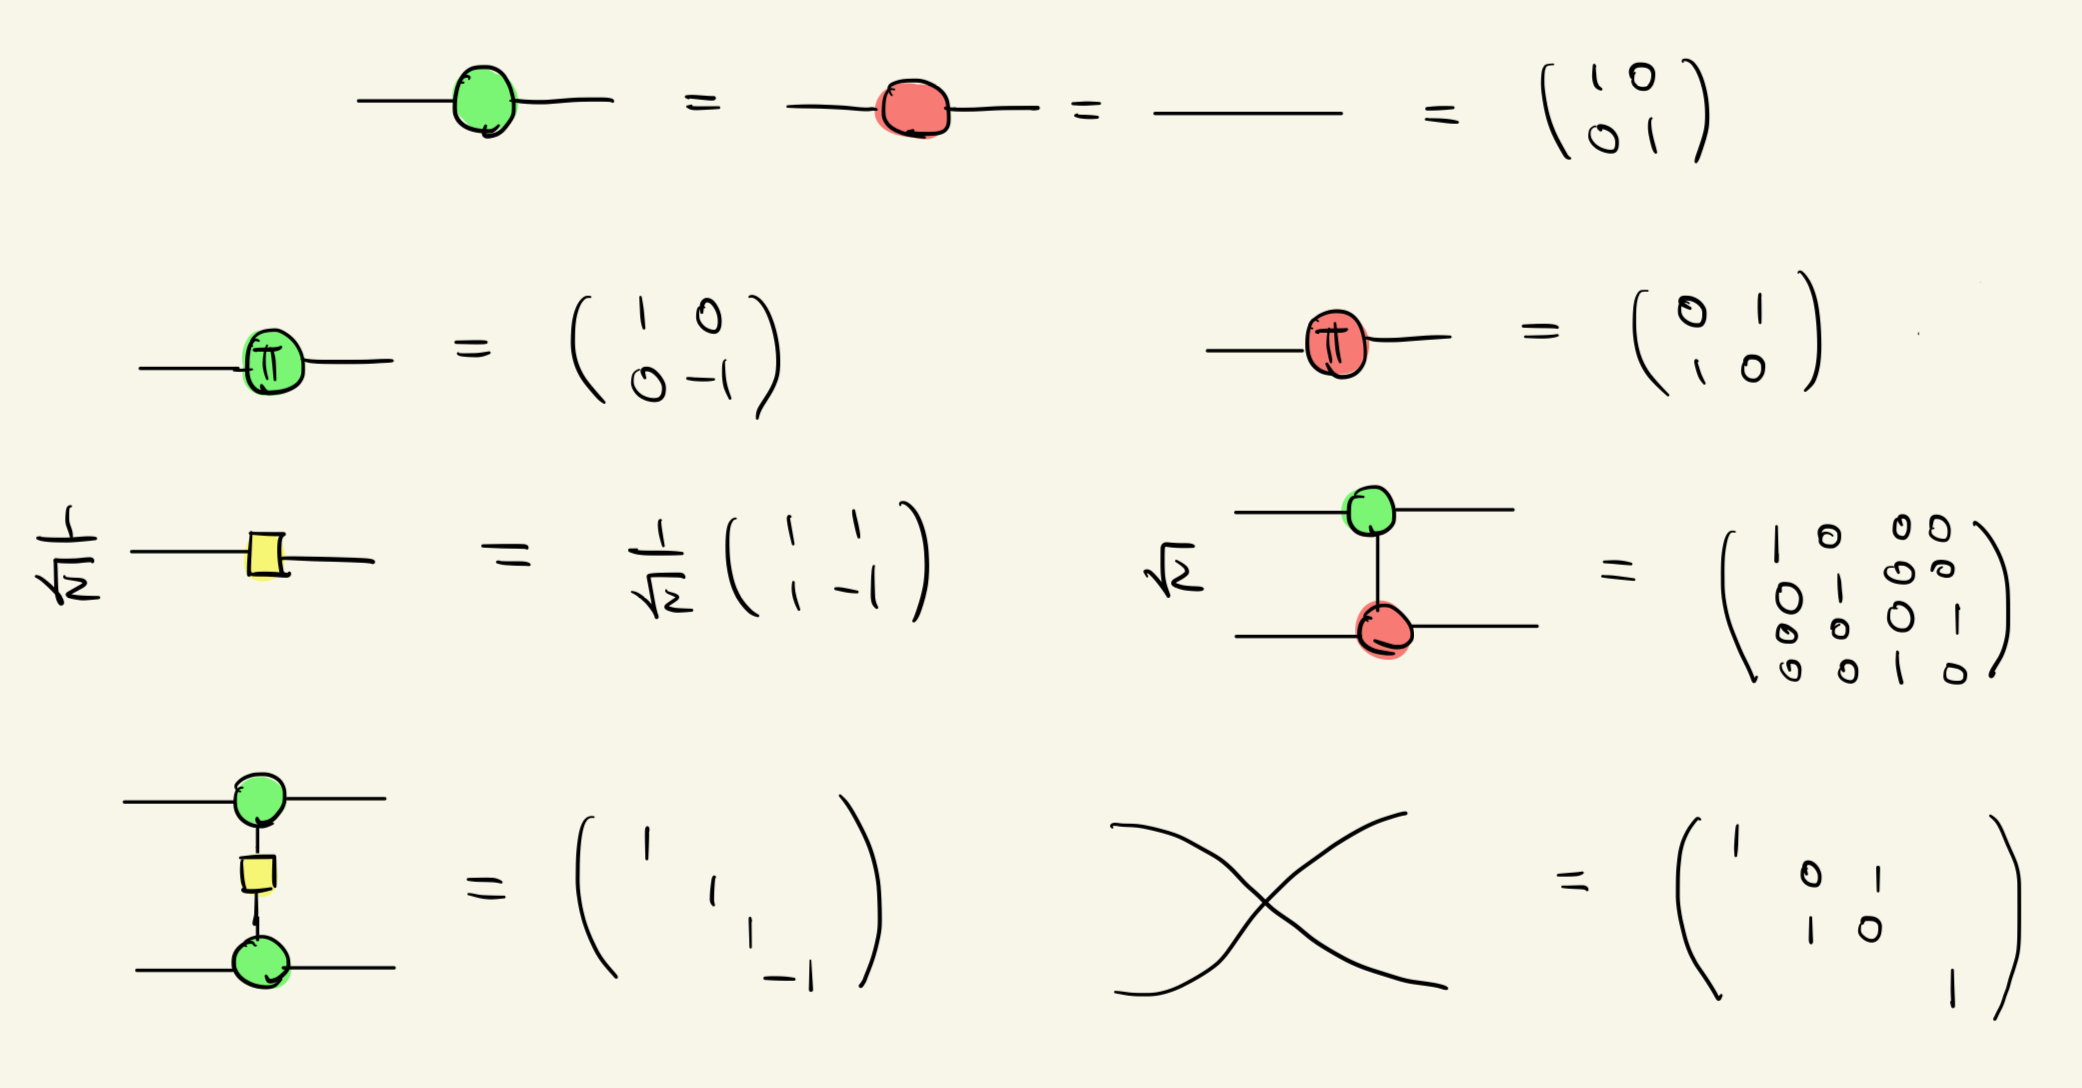
\includegraphics[width=.85\textwidth]{figures/zx_common_gates.PNG}
    \end{figure}
\end{frame}


\begin{frame}{Example - Control phase gates}
    % Write down the CCZ(theta) to illustrate the control nature of H 
    \begin{figure}
        \centering 
        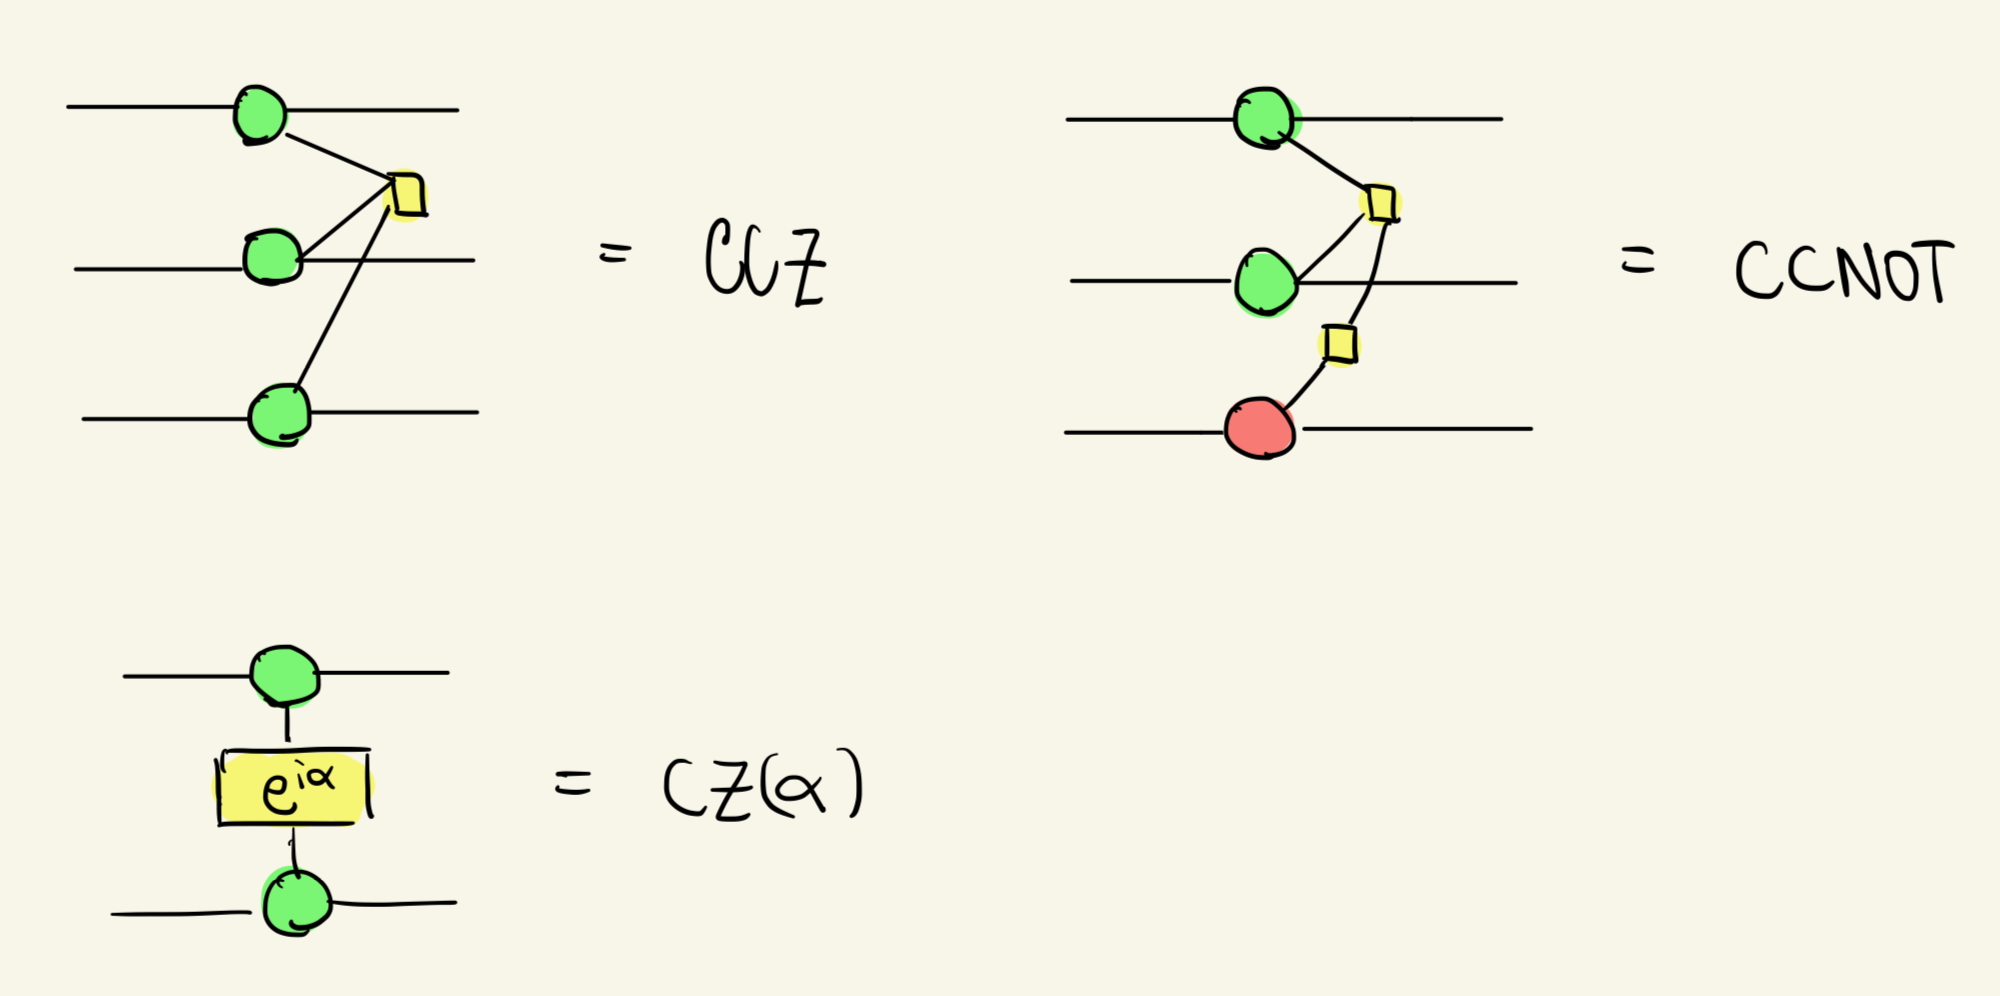
\includegraphics[width=.85\textwidth]{figures/zx_control_phases.PNG}
    \end{figure}
\end{frame}



%\begin{frame}{Example - Projector to triplet}
% Using the idea to write down the projector to triplet
%\end{frame}

\begin{frame}{Example - Convert diagrams to matrix}
    \begin{figure}
        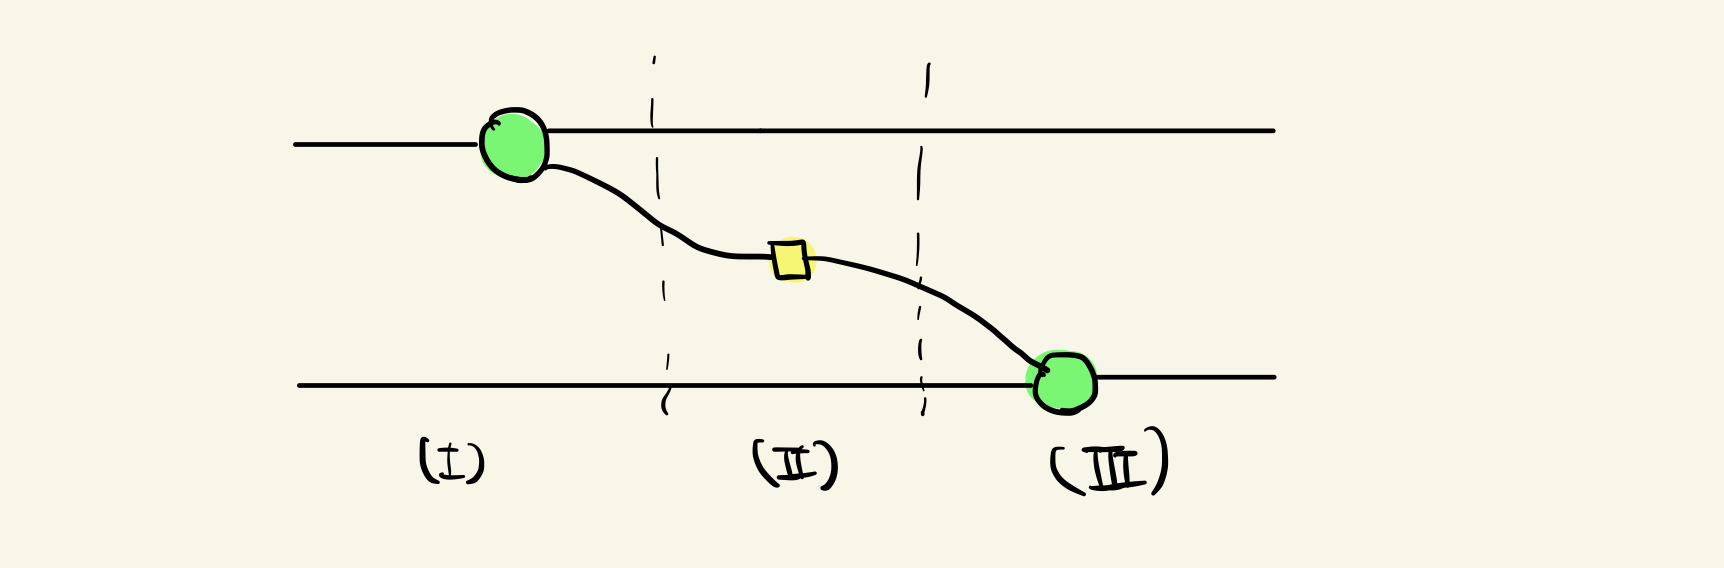
\includegraphics[width=.6\textwidth]{figures/zx_cz_to_matrix.PNG}
    \end{figure}
    \begin{align*}
        &\underbrace{\left[\begin{pmatrix}
            1 & 0\\
            0 & 1
        \end{pmatrix}\otimes \begin{pmatrix}
            1 & 0 & 0 & 0\\
            0 & 0 & 0 & 1
        \end{pmatrix}\right]}_{(III)}\underbrace{\left[\begin{pmatrix}
            1 & 0 \\
            0 & 1
        \end{pmatrix} \otimes \begin{pmatrix}
            1 & 1 \\
            1 & -1
        \end{pmatrix} \otimes \begin{pmatrix}
            1 & 0 \\
            0 & 1
        \end{pmatrix}\right]}_{(II)}\underbrace{\left[\begin{pmatrix}
            1 & 0\\
            0 & 0\\
            0 & 0\\
            0 & 1
        \end{pmatrix} \otimes \begin{pmatrix}
            1 & 0\\
            0 & 1
        \end{pmatrix} \right]}_{(I)} \\
        &= \text{diag}(1,1,1,-1) = \text{Control-Z}
    \end{align*}


 \end{frame}



\begin{frame}{ZX calculus over traditional MPS}
    \begin{itemize}
        \item \textbf{Complete}: Any equality of matrices with powers of $n$ can be derived purely diagrammatically using the rewritting rules\footnote{For pedagogical introduction to ZX rewritting rules, see \cite{zx_for_working_qcs} }
    \item \textbf{Only connectivity matters}: Two diagrams represent the same circuit if the underlying graphs are the same
    \item \textbf{Programmatic graph reduction}: Calculations can be done \underline{automatically} and \underline{exactly} by open source graph reduction packages, e.g. PyZX
    \end{itemize}
\end{frame}

\begin{frame}{Example - Applying CNOT to states}
    \begin{figure}
        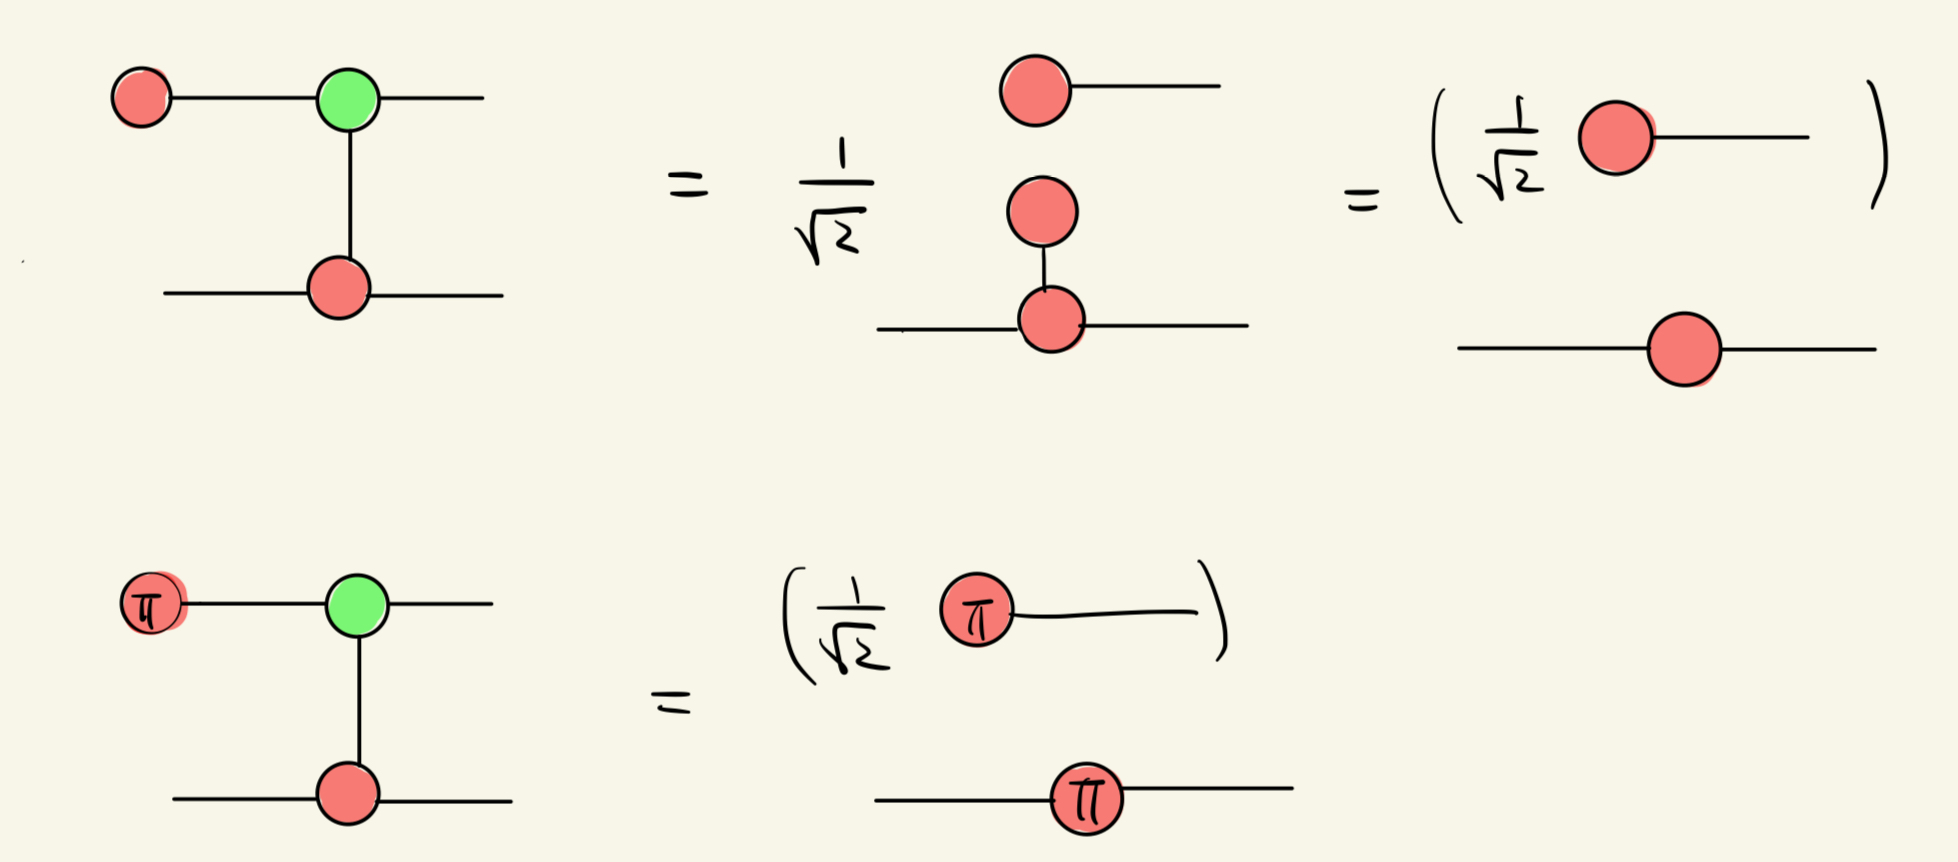
\includegraphics[width=.8\textwidth]{figures/zx_cnot_derivation.PNG}
    \end{figure}
\end{frame}

\begin{frame}{Example - 3 CNOT = Swap}
    \begin{figure}
        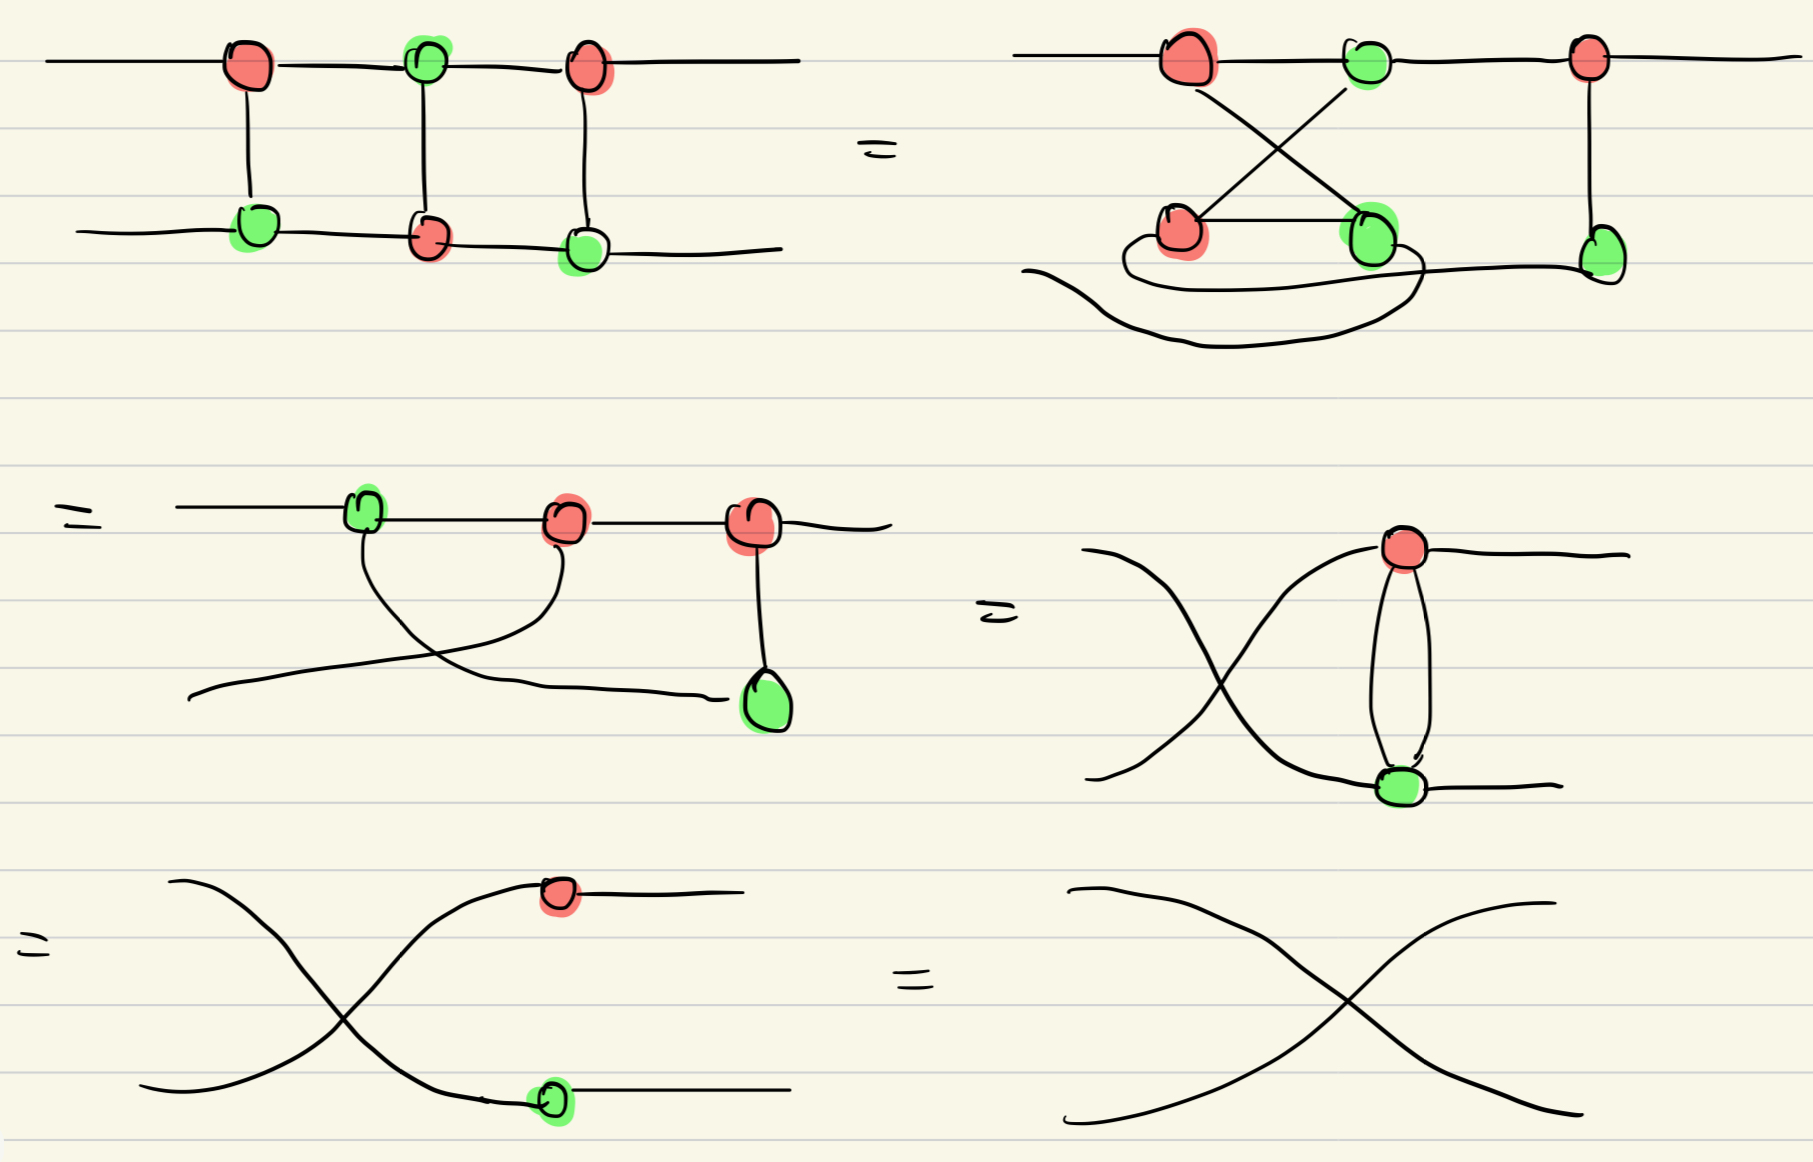
\includegraphics[width=.7\textwidth]{figures/zx_three_cnot_swap.PNG}
    \end{figure}
\end{frame}

\begin{frame}{Example - CX and CZ}
    \begin{figure}
        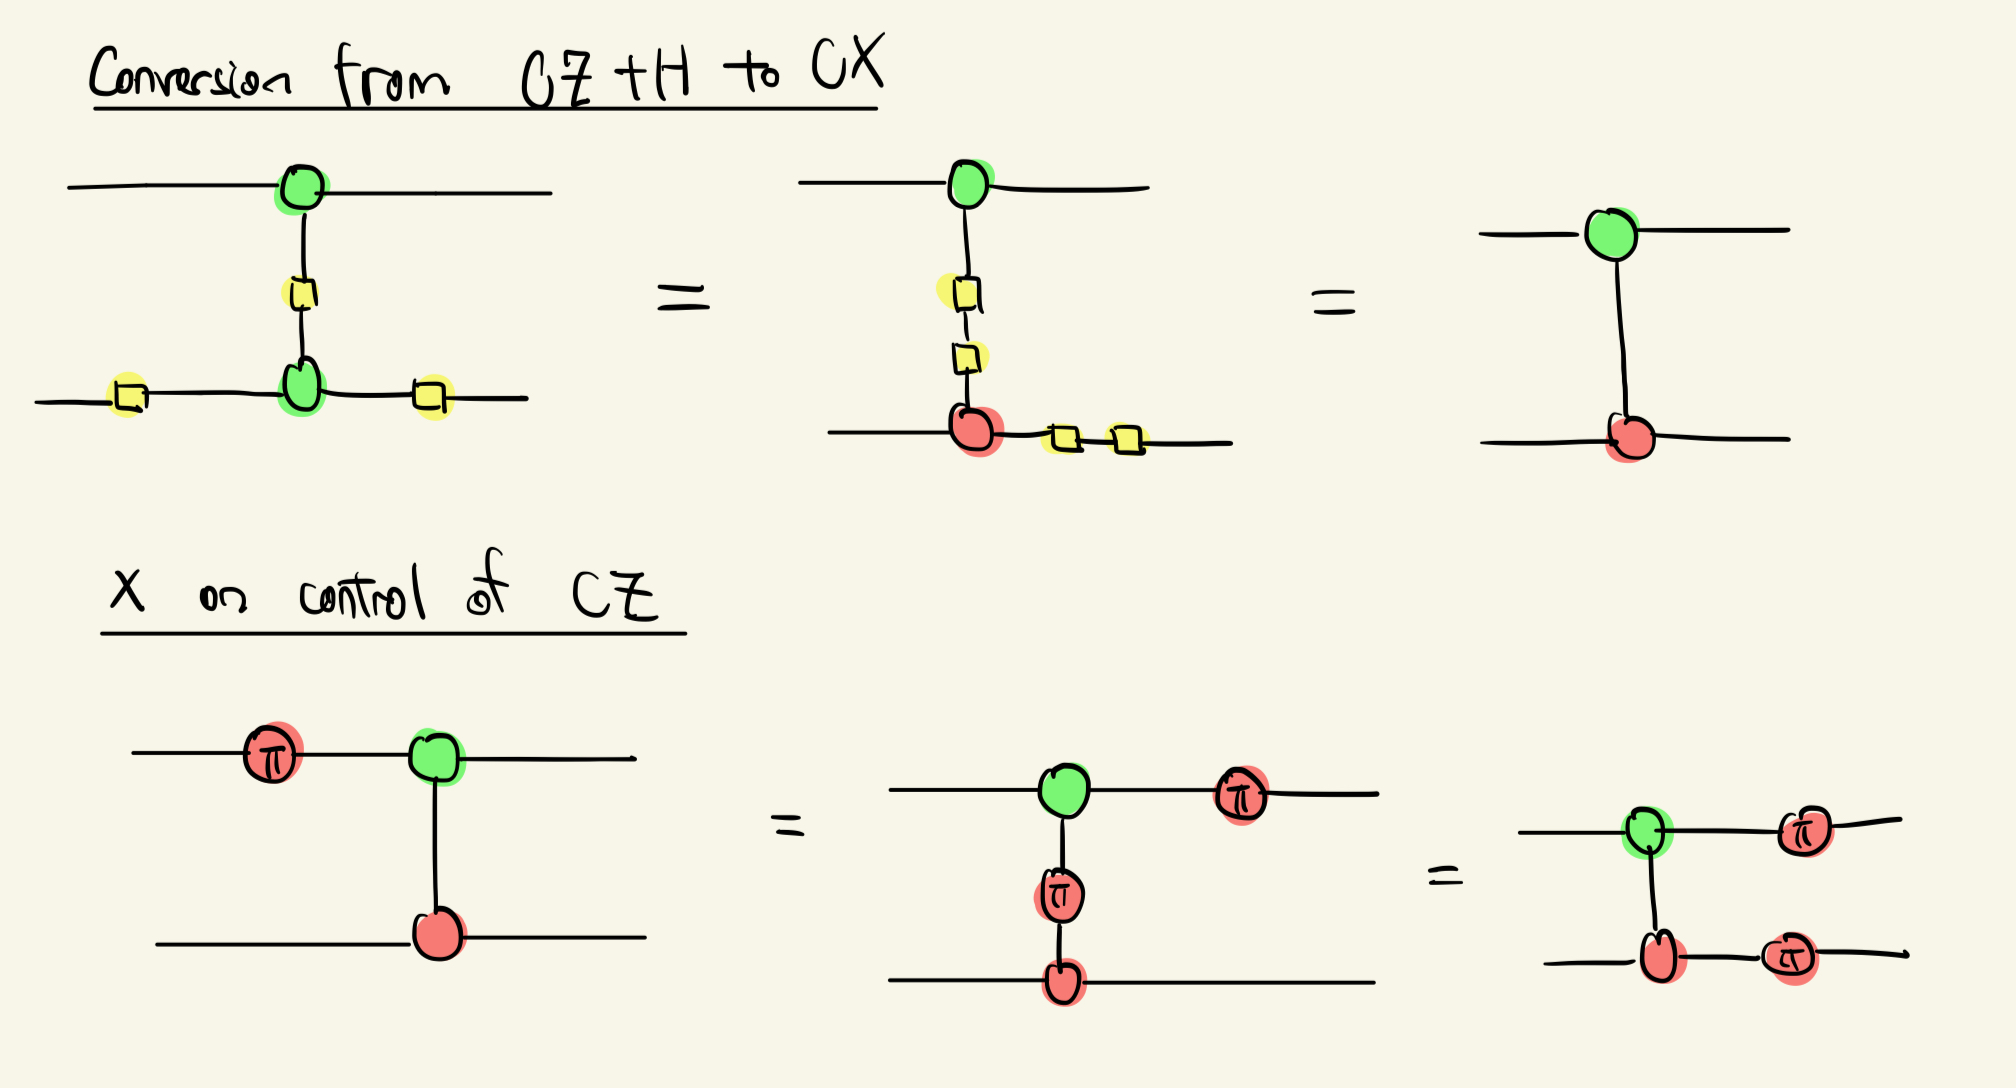
\includegraphics[width=.7\textwidth]{figures/zx_cx_cz_identities.PNG}
    \end{figure}
\end{frame}

\begin{frame}{Example - Bell state preparation \& Inverse}
    \begin{figure}
        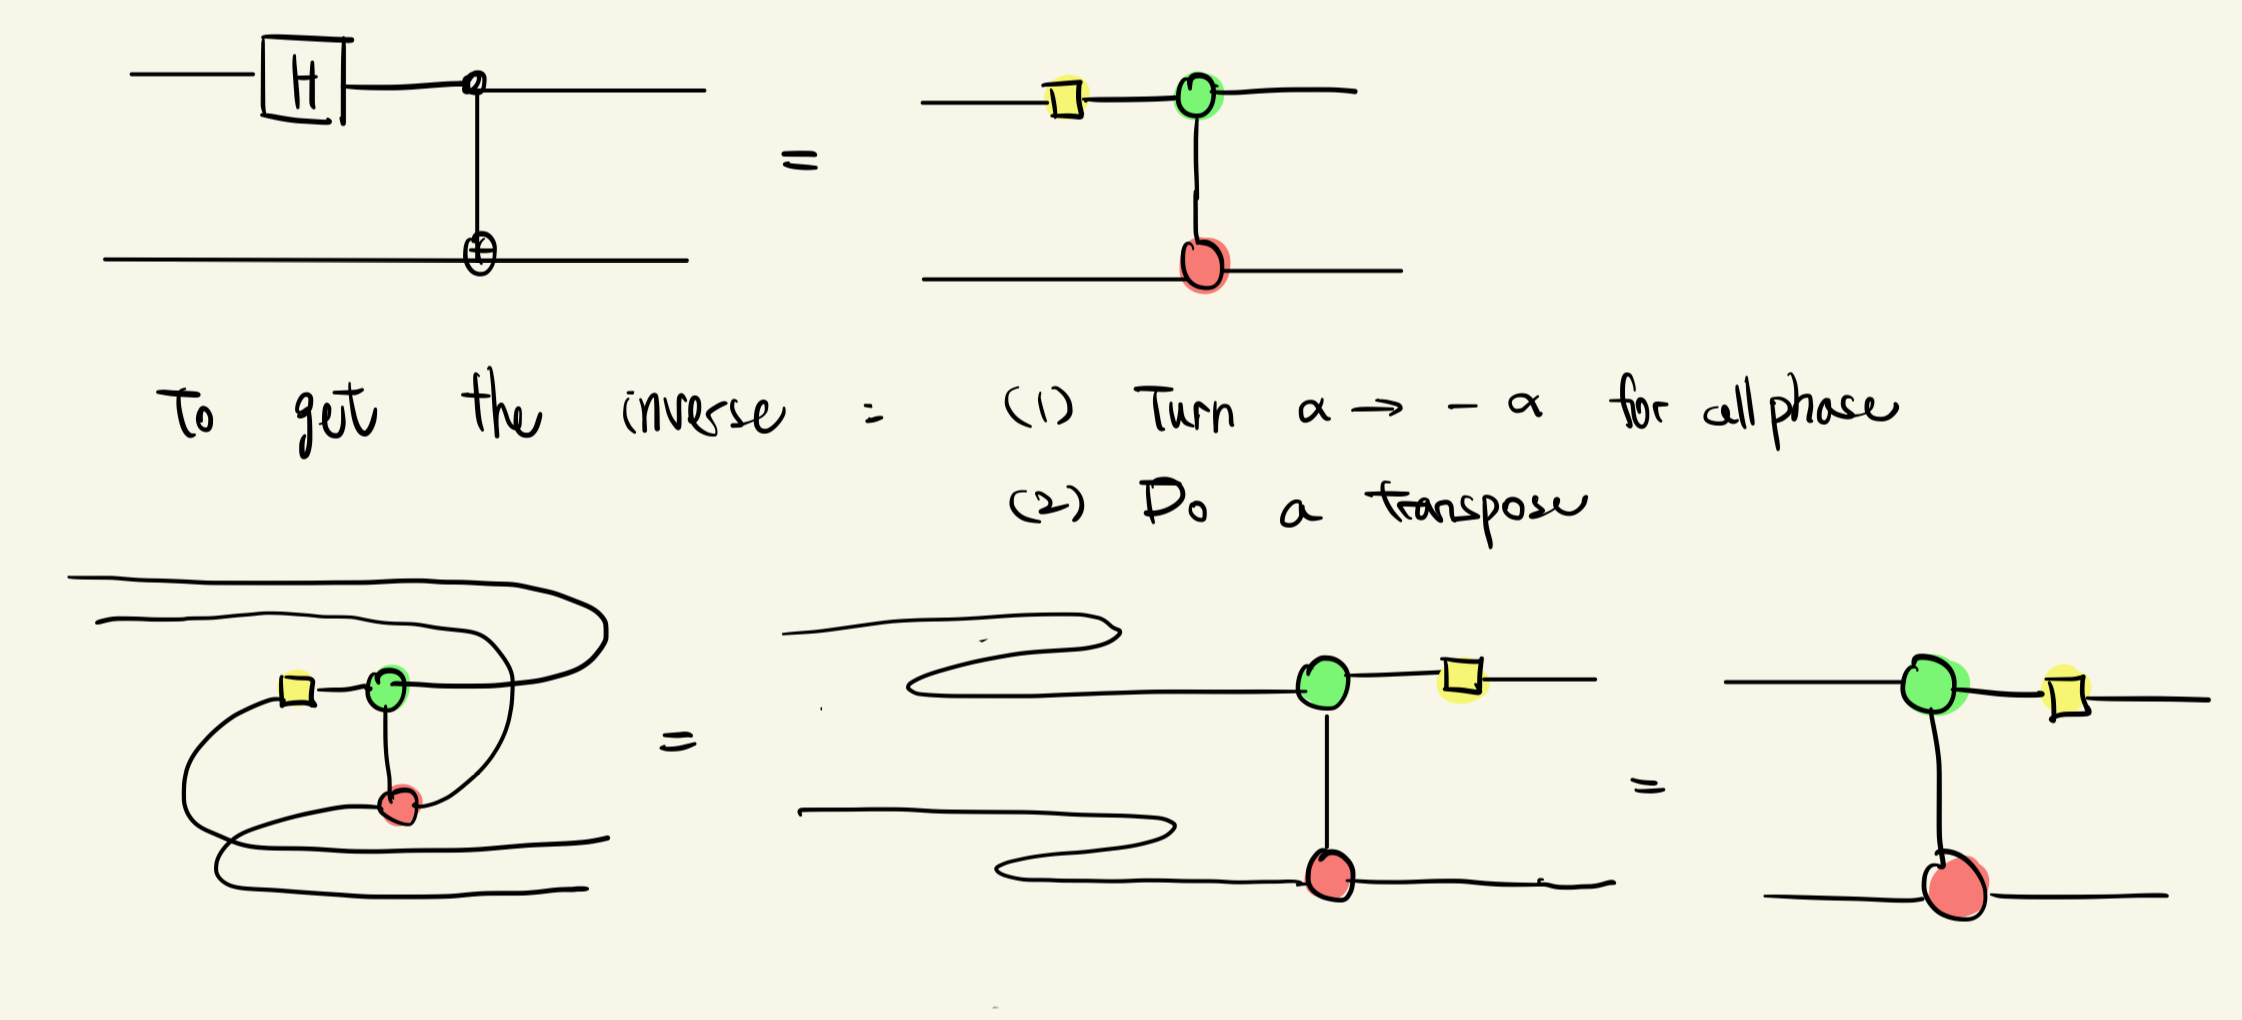
\includegraphics[width=.8\textwidth]{figures/zx_bell_state_prep.PNG}
    \end{figure}
\end{frame}

\begin{frame}{Example - Project away $\ket{11}$}
    \begin{figure}
        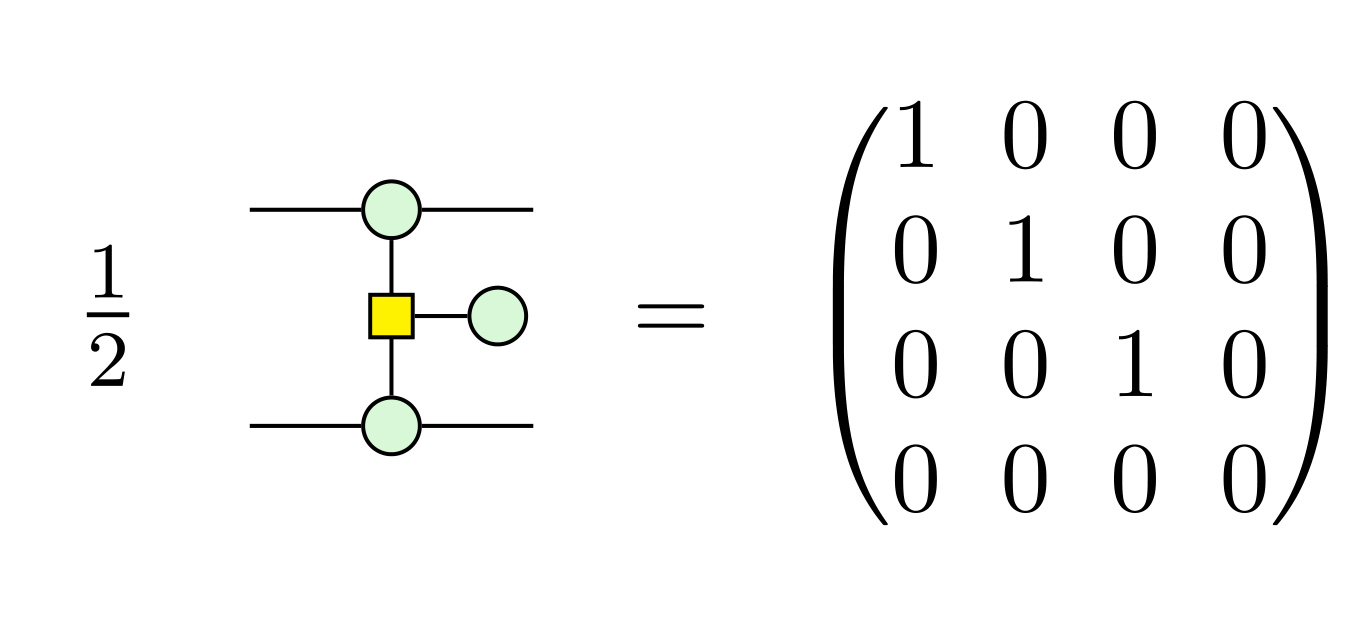
\includegraphics[width=.8\textwidth]{figures/zx_remove_oneone.png}
    \end{figure}
    \footnote{Note the control nature of the multi-leg H-box}
\end{frame}



\makesection{1D AKLT as ZX diagrams}
\begin{frame}{AKLT GS - Covalent bonds}
\begin{itemize}
    \item Take bell state, apply $X_2$ and $Z_1$ 
\end{itemize}
\begin{figure}
    \centering
    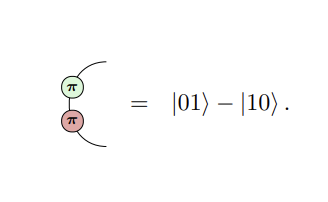
\includegraphics[width=.5\textwidth]{figures/covalent_bond.png}
\end{figure}
\end{frame}

\begin{frame}{AKLT GS - Spin-1 projector}
    \begin{itemize}
        \item The Bell state preparation circuit $\ket{11} \to \ket{\Psi^{-}}= \left(\ket{01} - \ket{10}\right)/\sqrt{2}$
        \item \underline{Strategy:} $\text{(Bell prep)}^{\dagger} \circ (\text{Project out } \ket{11}) \circ \text{(Bell prep)}^{\dagger}$
    \end{itemize}
    \begin{figure}
        \centering
        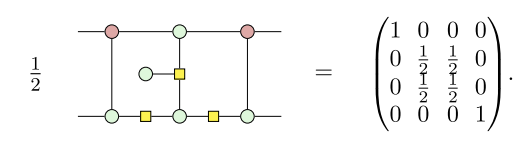
\includegraphics[width=.8\textwidth]{figures/spin_one_proj.png}
    \end{figure}
\end{frame}

\begin{frame}
    To construct the AKLT state, we first write down the valence bond pairs
    \begin{figure}
        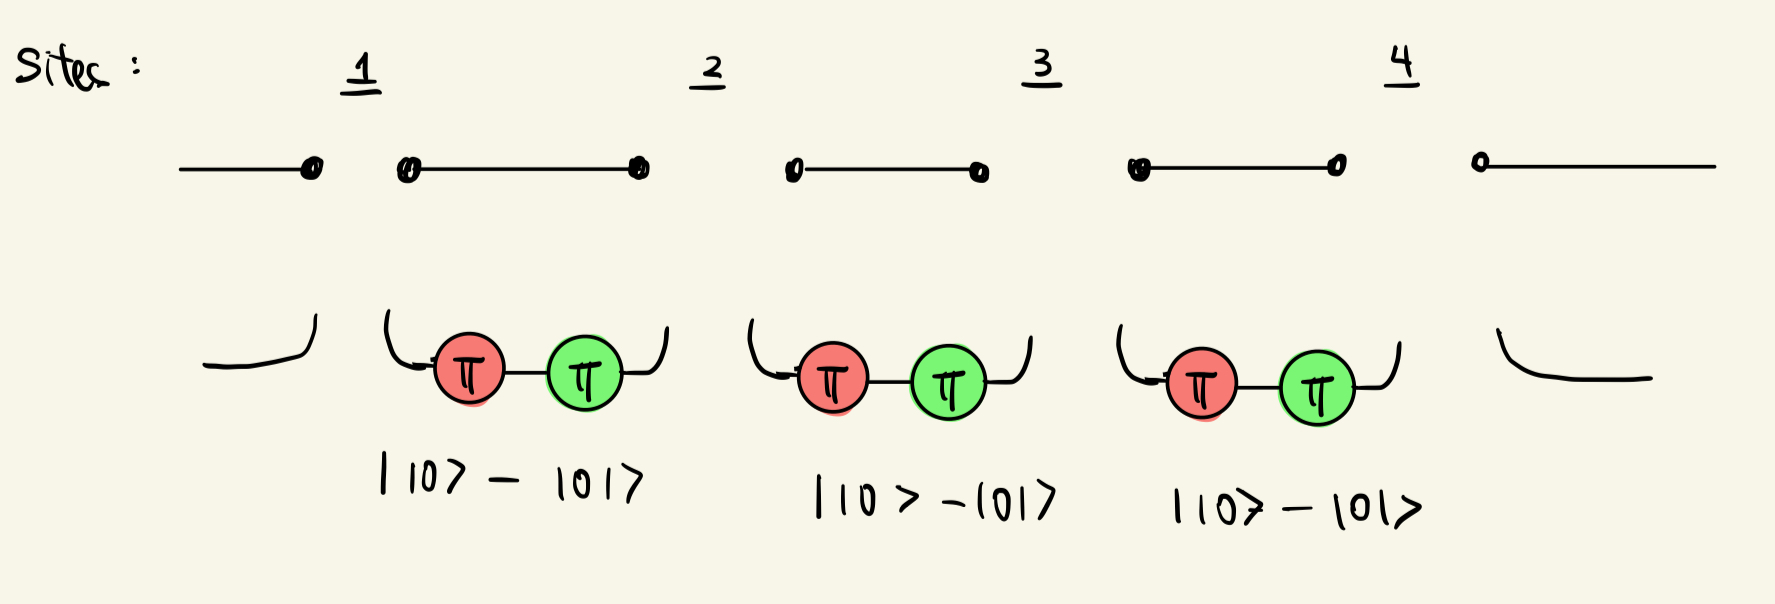
\includegraphics[width=0.9\textwidth]{figures/aklt_valence_bond.PNG}
    \end{figure}
\end{frame}

\begin{frame}
    We then apply the porjector to project onto the spin-1 subspace 
    \begin{figure}
        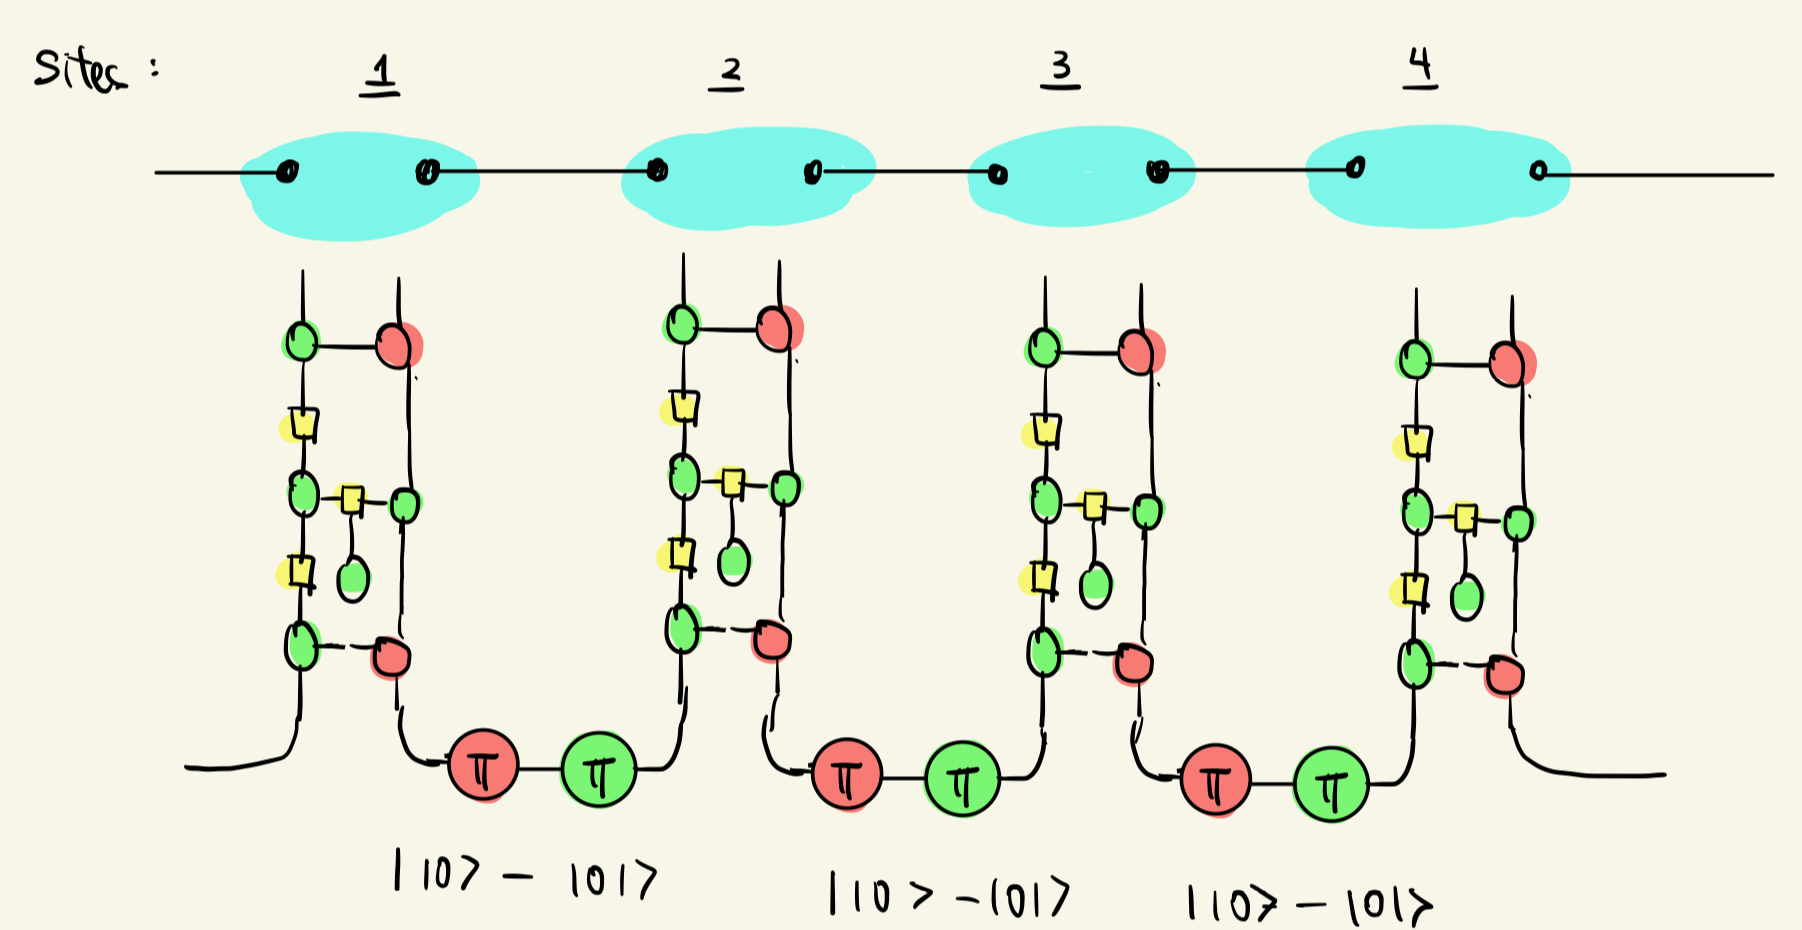
\includegraphics[width=0.9\textwidth]{figures/aklt_valence_bond_plus_projector.PNG}
    \end{figure}
    The dangling wires at the edge of the chain signifies the 4-fold degeneracies 
\end{frame}

\begin{frame}
    \textbf{Recovering MPL matrices by contraction} 
    \begin{figure}
        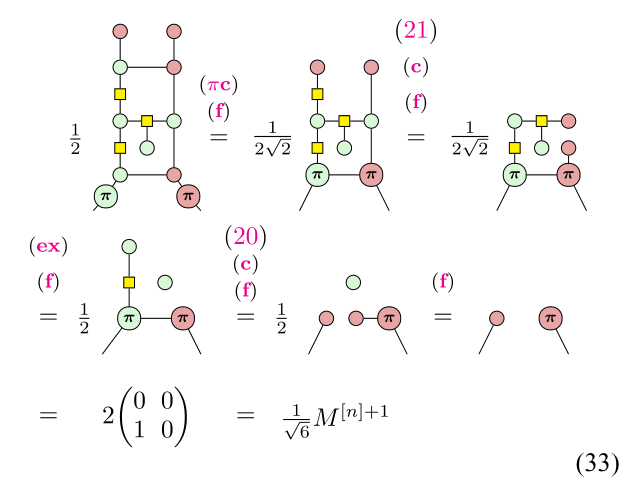
\includegraphics[width=.8\textwidth]{figures/mpl_matrix_graph_reduction_m1.PNG}
    \end{figure}
\end{frame}



\begin{frame}{Demonstrating hidden string order}
    \begin{figure}
        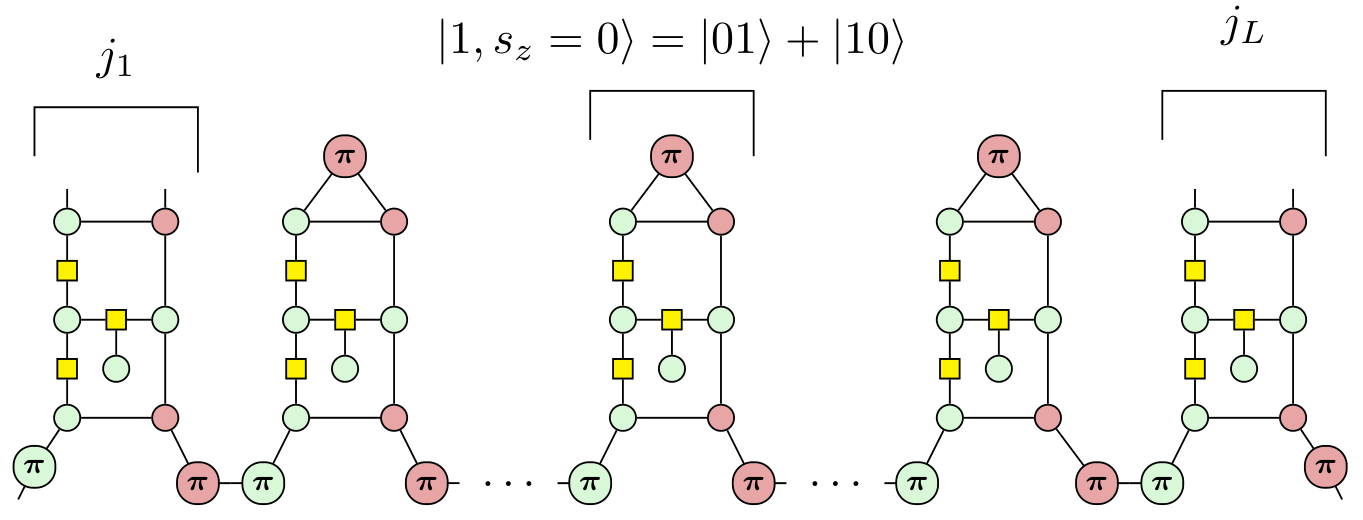
\includegraphics[width=.8\textwidth]{figures/zx_hidden_string_order_strategy.png}
    \end{figure}
\end{frame}

\begin{frame}
    Simplify the repeating block in the middle, we get the following figure
    \begin{figure}
        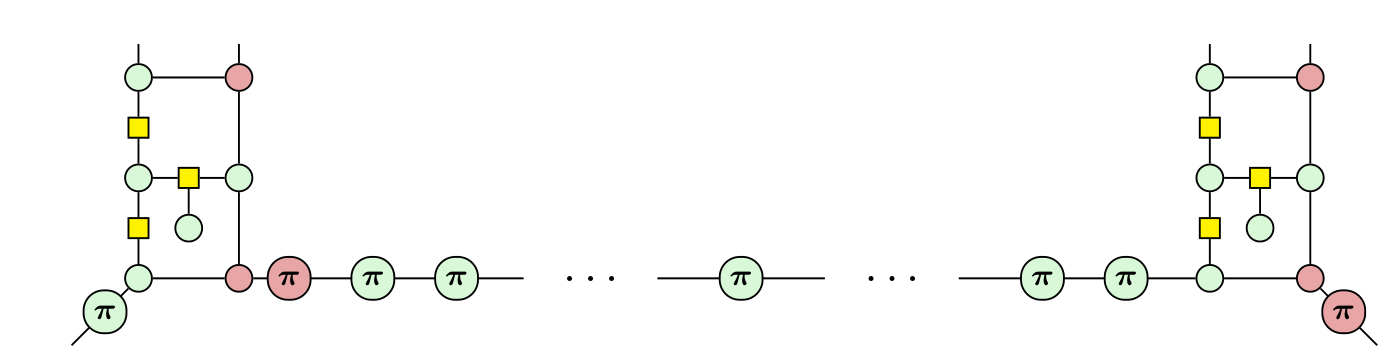
\includegraphics[width=\textwidth]{figures/zx_hidden_string_order_simplify_zero_projections.png}
    \end{figure}
    \begin{figure}
        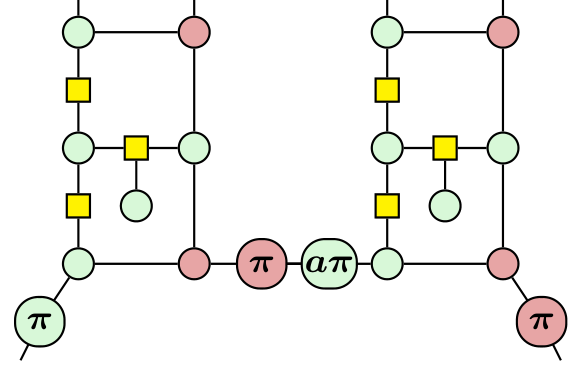
\includegraphics[width=.3\textwidth]{figures/zx_hidden_string_order_simplify_zero_projections_final.png}
    \end{figure}
    Plugging in $\pm 1$ on both sides shows that the state vanishes if $j_1 = j_L$ does not otherwise (Work out an example that gives 0)
\end{frame}


\begin{frame}{Berry phase computation}
    \begin{itemize}
        \item Recall the Berry phase is calculated using 
        $$\gamma = -i \int_{0}^{2\pi} \frac{\braket{\psi_\theta| \partial_\theta |\psi_\theta}}{\braket{\psi_\theta|\psi_\theta}} d\theta$$
        where the chain is twisted at the end
        \item We calculate the phase directly by representing both $\ket{\psi_\theta}$ and $\bra{\psi_\theta}$ as ZX diagrams and doing all the contractions diagrammatically
    \end{itemize}
\end{frame}

\begin{frame}
    \begin{figure}
        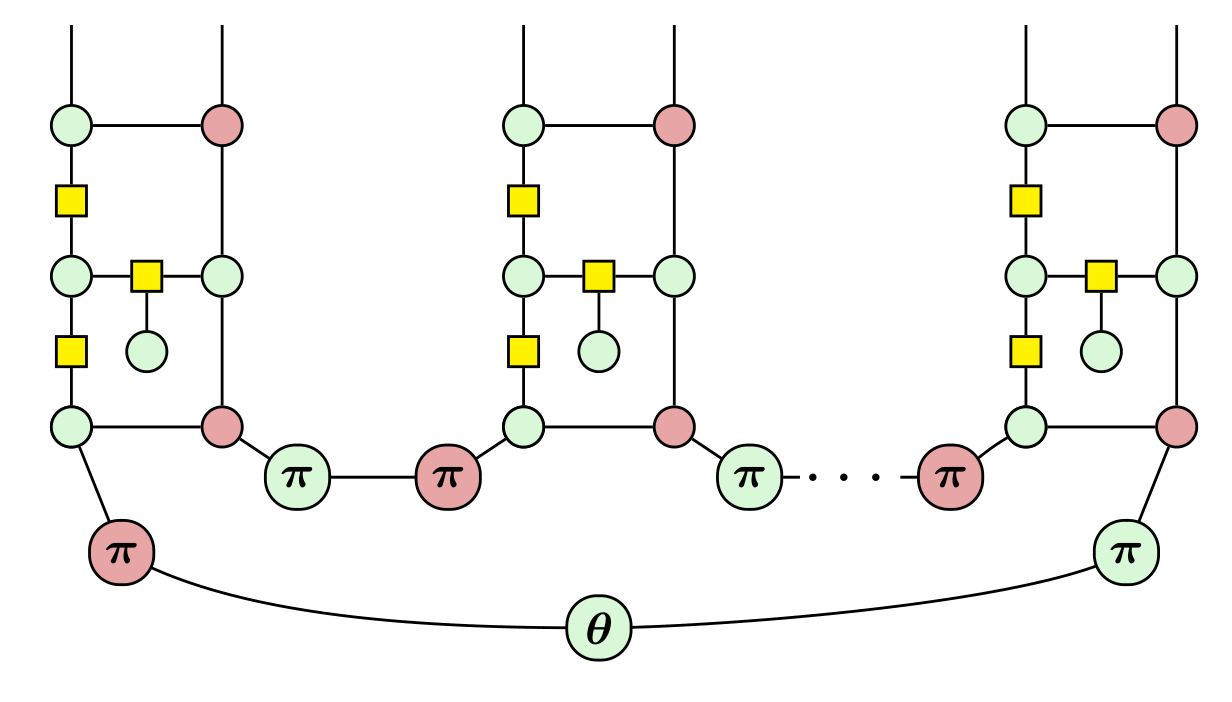
\includegraphics[width=.8\textwidth]{figures/zx_berry_phase_state.png}
    \end{figure}
    
\end{frame}
\begin{frame}
    The integral is therefore
    \begin{figure}
        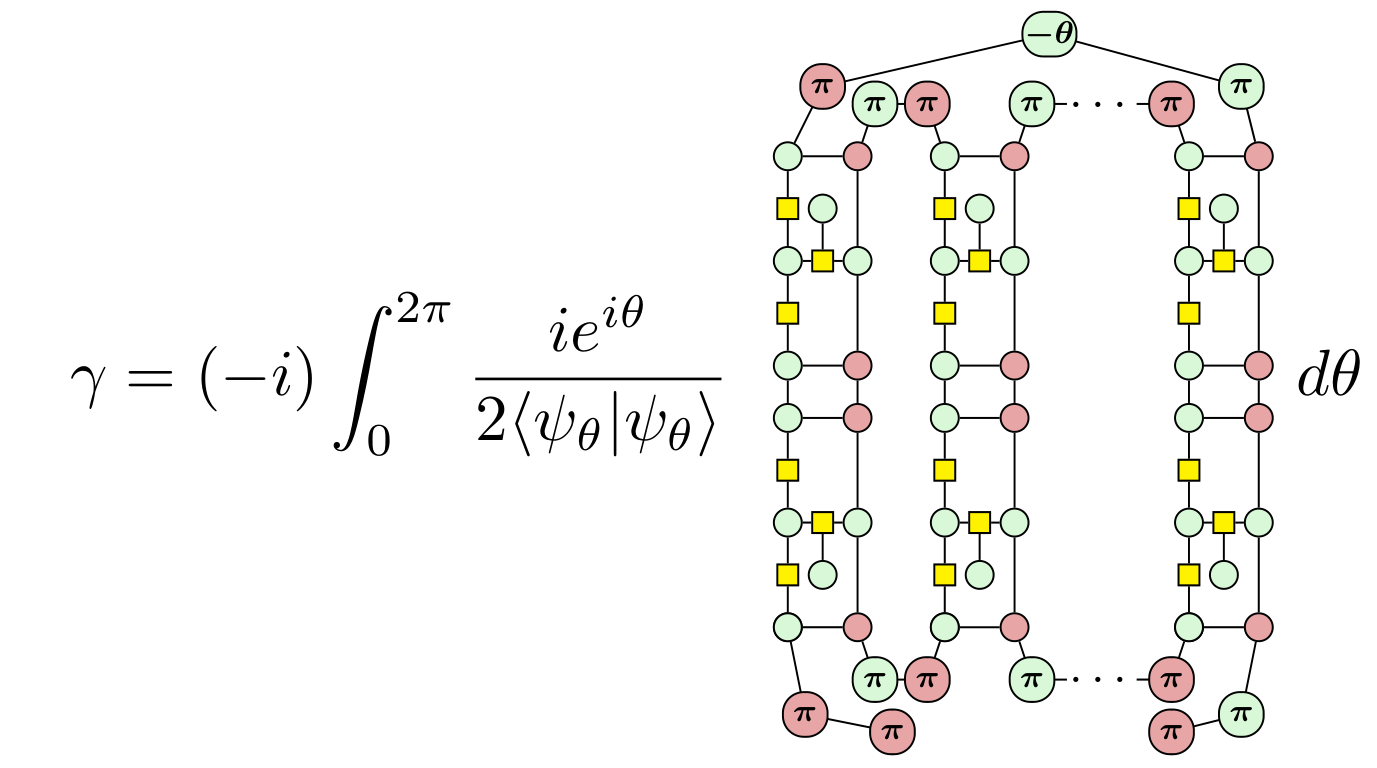
\includegraphics[width=.8\textwidth]{figures/zx_berry_phase_integral.png}
    \end{figure}
\end{frame}

\begin{frame}
    Skipping the simplification steps, the result can be evaluated exactly as
    \begin{align*}
        \gamma &= \frac{1}{2}\int_{0}^{2\pi} \frac{2(-1)^N e^{i\theta} + 3^N + (-1)^N}{2(-1)^N \cos \theta + 3^N + (-1)^N} d\theta\\
        &= \frac{1}{2} \int_{0}^{2\pi} \frac{g e^{i\theta} + 1}{g\cos \theta +1} d\theta = \boxed{\pi}
    \end{align*}
    where $g = \frac{2(-1)^N}{3^N+(-1)^N}$, and $N$ is the length of the chain.
    Thus, the direct computation shows that $\boxed{\gamma = \pi}$ holds for all finite length 1D AKLT chains.

\end{frame}


\makesection{2D AKLT States as ZX diagram}

\begin{frame}{2D AKLT states on honeycomb lattice}
    %Spin-3/2 per site; GS constructed by valence bonds on edge + projection

    \begin{figure}
        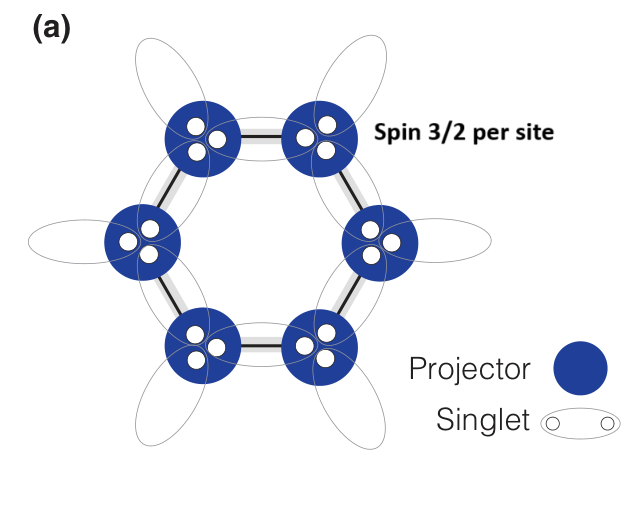
\includegraphics[width=.6\textwidth]{figures/two_dim_aklt_on_honeycomb.png}
    \end{figure}
\end{frame}

\begin{frame}{Spin-3/2 Projector}
    \begin{figure}
        \centering
        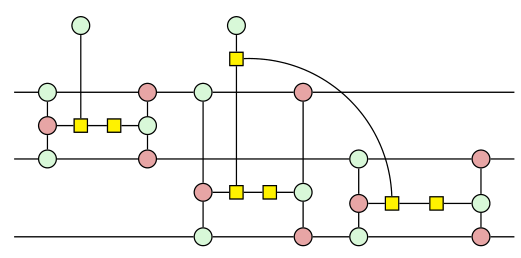
\includegraphics[width=.8\textwidth]{figures/spin_three_half_projector.png}
    \end{figure}
\end{frame}

\begin{frame}
    \begin{figure}
        \centering
        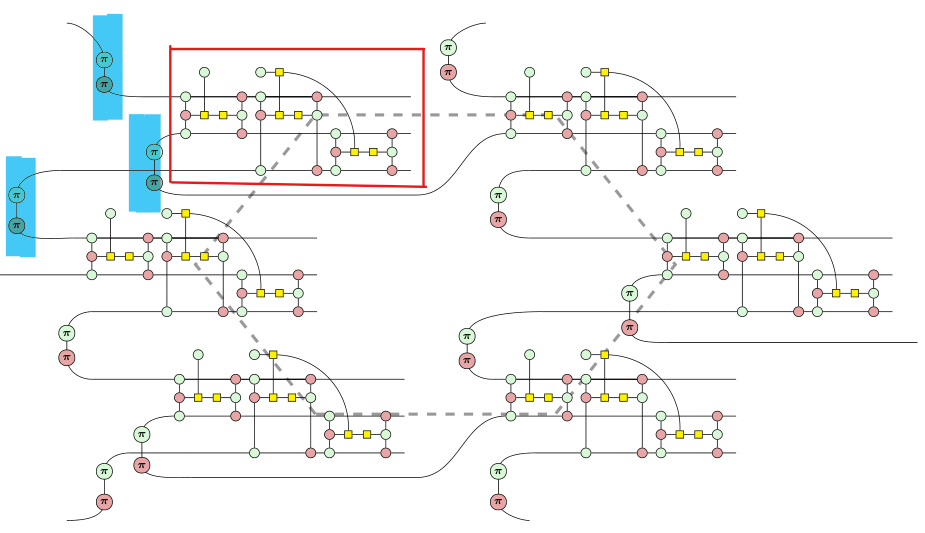
\includegraphics[width=.9\textwidth]{figures/zx_two_dim_aklt_on_honeycomb.png}
    \end{figure}
\end{frame}

\begin{frame}{Previously known facts about this states} 
    \begin{itemize}
        \item The state can be reduced into a graph state under suitable measurement operations \cite{wei2011_aklt_honeycomb}
        \item The measurement is a joint measurement of the 3 qubit on each site
        \begin{align*}
            E_z &= \frac{2}{3} \left(\ket{000}\bra{000}+\ket{111}\bra{111}\right) \\
            E_x &= \frac{2}{3} \left(\ket{+++}\bra{+++}+\ket{---}\bra{---}\right) \\
            E_y &= \frac{2}{3} \left(\ket{iii}\bra{iii}+\ket{-i-i-i}\bra{-i-i-i}\right)  
        \end{align*}
        where $\ket{0},\ket{+},\ket{i}$ are the eigenstates of the $Z,X,Y$ operators \footnote{Note that $E^\dagger_x E_x+E_y^\dagger E_y+ E^\dagger_zE_z = P_{3/2}$}
    \end{itemize}
\end{frame}

\begin{frame}
    \textbf{Graph reduction rules:}
    \begin{itemize}
        \item After measurement is performed, apply the following graph reduction rules
        \begin{enumerate}[(i)]
            \item Merge neighboring sites with same POVM outcomes
            \item Cut pairs of edges that connects two vertices
        \end{enumerate}
        \item The merged sites are called a \textit{domain} and represent a single-logical qubit
    \end{itemize}
    \vspace{.5cm}
    \textbf{Reasons for the rules to hold:}
    \begin{enumerate}
        \item Neighboring sites are antiferromagnetic, so if both of them are $S_a=\pm 3/2$, one can only have combinations of form $\ket{3/2, -3/2,\cdots}_{12}$ or $\ket{-3/2, 3/2,\cdots}_{12}$ 
        \item Let $m$ be the multiplicity of an edge, the inferred graph state stabilizer generators is of form $X_u Z_v^m$.\footnote{To be honest I can't follow this part of the argument} Since $Z^2=I$, we can remove all but one edge.
    \end{enumerate}
    \vspace{.5cm}
    \textbf{Universal Quantum Resource: }The construction above gives a cluster state in thermodynamic limit, which is a univeral quantum resource.
\end{frame}

\begin{frame}{Graph state in ZX calculus}
    \begin{figure}
        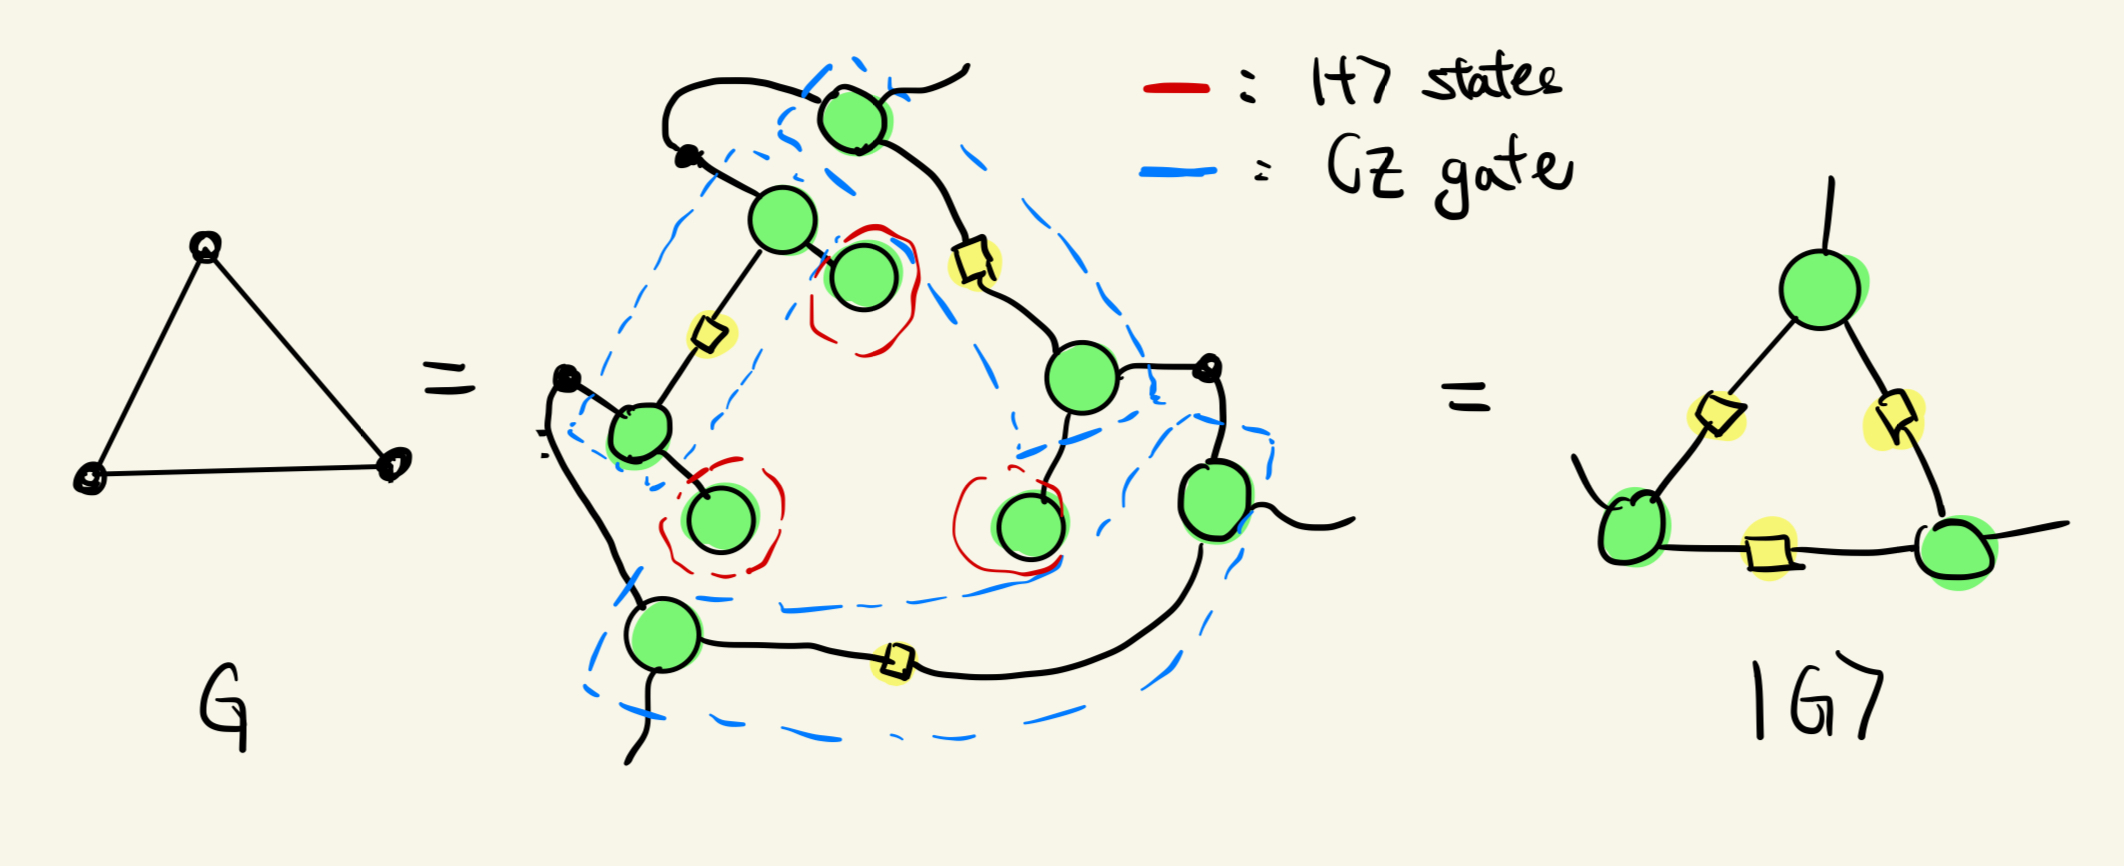
\includegraphics[width=.95\textwidth]{figures/zx_graph_state.PNG}
    \end{figure}
\end{frame}


\begin{frame}
    \textbf{Graph state reduction proof (ZX calculus):}\\ We first write down the POVM operators
    \begin{columns}
        \begin{column}{0.45\textwidth}
          \begin{figure}
            \centering
            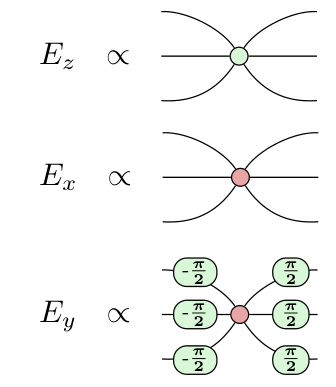
\includegraphics[width=.8\textwidth]{figures/povm_spiders_three_in_three_out.png}
          \end{figure}
        \end{column}
        \begin{column}{0.45\textwidth}  %%<--- here
            \begin{figure}
                \centering
                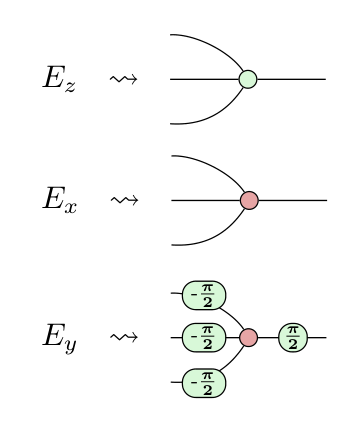
\includegraphics[width=.8\textwidth]{figures/povm_spiders_three_in_one_out.png}
              \end{figure}
            \end{column}
        \end{columns}
\end{frame}

\begin{frame}
    All of these operators are symmetric under permutation, so they "annihilate" the spin-3/2 projector and connects to the singlet directly
    \begin{figure}
        \centering
        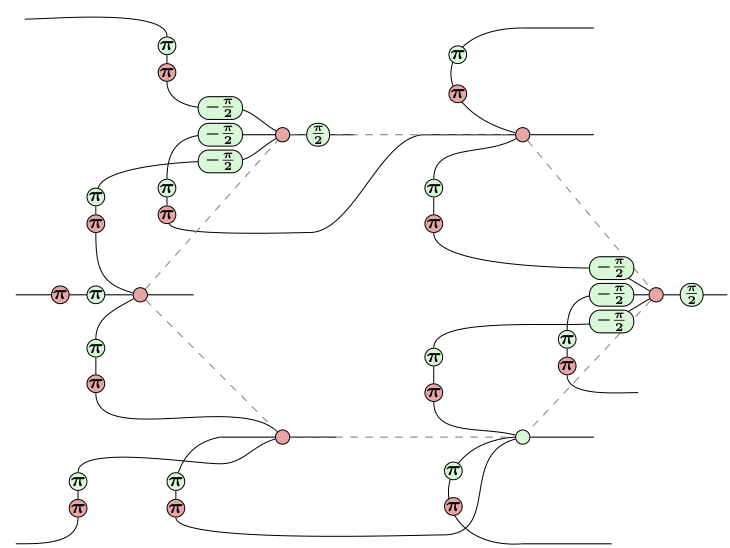
\includegraphics[width=.67\textwidth]{figures/povm_measurment_simplified.png}
    \end{figure}
\end{frame}

\begin{frame}
    \textbf{Using known results on Clifford states:}
    \begin{itemize}
        \item The diagram only contains contain any higher-arity H-boxes, and the only phases that appear are multiples of $\pi/2$
        \item It is a so-called Clifford state, which can be presented as a graph state with single-qubit Clifofrd unitaries on its outputs. QED.
        \item We can also do it explicitly
    \end{itemize}
    
\end{frame}

\begin{frame}
    \textbf{Explicit graph reduction}\\
    \begin{itemize}
        \item First rewrite the edges so that we have a $(\pi)-(\pi)$ in the output edges
        \begin{figure}
            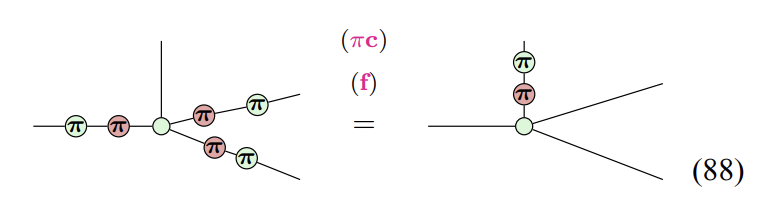
\includegraphics[width=.8\textwidth]{figures/zx_graph_reduce_1.png}
        \end{figure}
        With that we can redefine our basis and eliminate those phases.
        \item We can then merge all the vertices with same color, this is the same as Rule 1 in \cite{wei2011_aklt_honeycomb}
    \end{itemize}
\end{frame}

\begin{frame}
    \begin{itemize}
        \item We can then pull out hadamard gates from red vertices to make our states manifestly "graph-like"
        \begin{figure}
            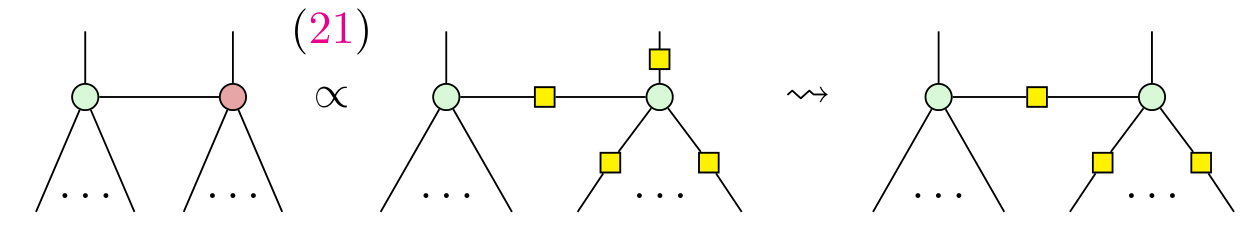
\includegraphics[width=.8\textwidth]{figures/zx_graph_reduce_2.png}
        \end{figure}
        \vspace{1cm}
        \item We can then remove edges with multiplicity $m>1$ by using the Hopf rule
        \begin{figure}
            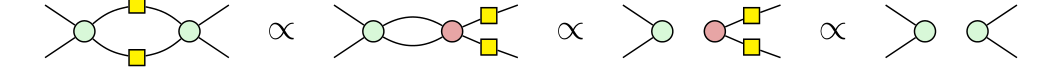
\includegraphics[width=.8\textwidth]{figures/zx_graph_reduce_3.png}
        \end{figure}
        This is basically Rule 2 in \cite{wei2011_aklt_honeycomb}
    \end{itemize}
\end{frame}

\begin{frame}
\begin{figure}
    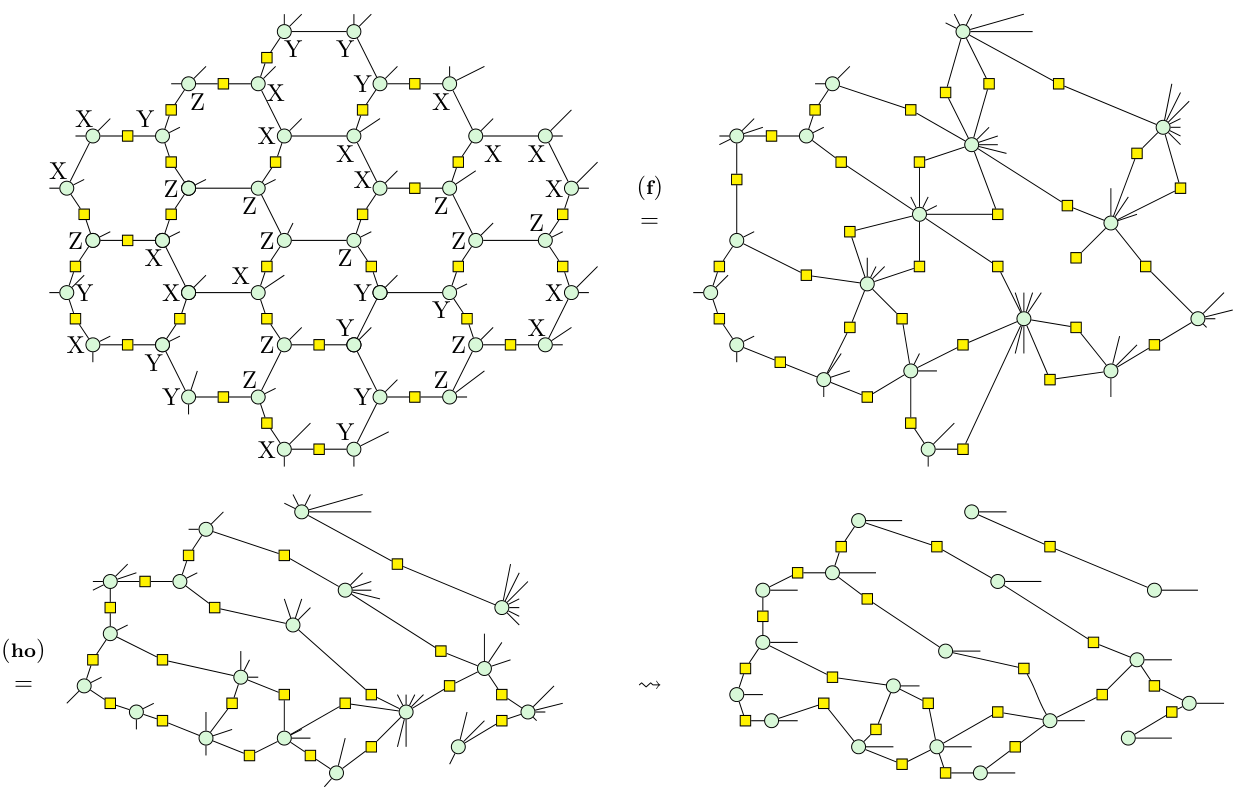
\includegraphics[width=0.9\textwidth]{figures/zx_graph_reduce_4.png}
\end{figure}
\end{frame}


\makesection{Using PyZX}
\begin{frame}{About PyZX}
    \begin{itemize}
        \item PyZX is an open-source packages for ZXH calculus
        \item Allows you to construct circuits and graphs directly
        \item Also supports automatic graph simplification
        \item Repo link: \href{https://github.com/Quantomatic/pyzx}{https://github.com/Quantomatic/pyzx}
    \end{itemize}
    \begin{figure}
        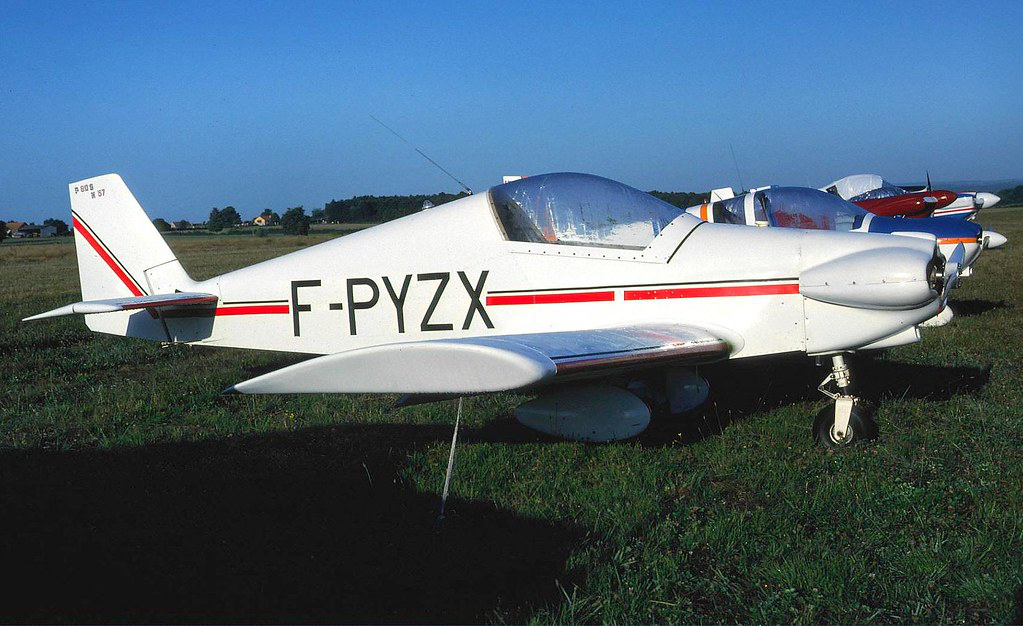
\includegraphics[width=.5\textwidth]{figures/fpyzx.png}
    \end{figure}
\end{frame}

\begin{frame}{Graphical reduction with PyZX}
    \vspace{2.5cm}
    \begin{quotation}
        "Talk is cheap. Show me the code." - Linus Torvalds
    \end{quotation}

\end{frame}
%\begin{frame}
%    \textbf{Performing the reduction using PyZX}\\
%    \vspace{.5cm}
%    We first write down the projector (with a hidden prefactor $1/2$)
%    \begin{figure}
%        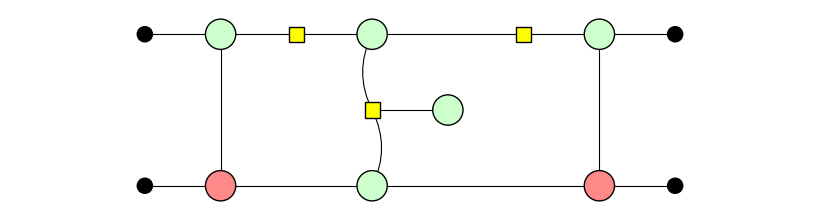
\includegraphics[width=.8\textwidth]{figures/pyzx_spin_one_projector.png}
%    \end{figure}
%    which has the matrix form:
%    \begin{align*}
%        \begin{pmatrix}
%            1 & 0 & 0 & 0 \\ 
%            0 & 2^{-1} & 2^{-1} & 0 \\ 
%            0 & 2^{-1} & 2^{-1} & 0 \\ 
%            0 & 0 & 0 & 1
%            \end{pmatrix}
%    \end{align*}
%\end{frame}


%\begin{frame}
%    We can stack the figures vertically using the \texttt{@} operator
%\end{frame}



\appendix
%------------------------------------------------
\makesection{Appendix }
\begin{frame}{ZX calculus rewritting rules}
\begin{figure}
    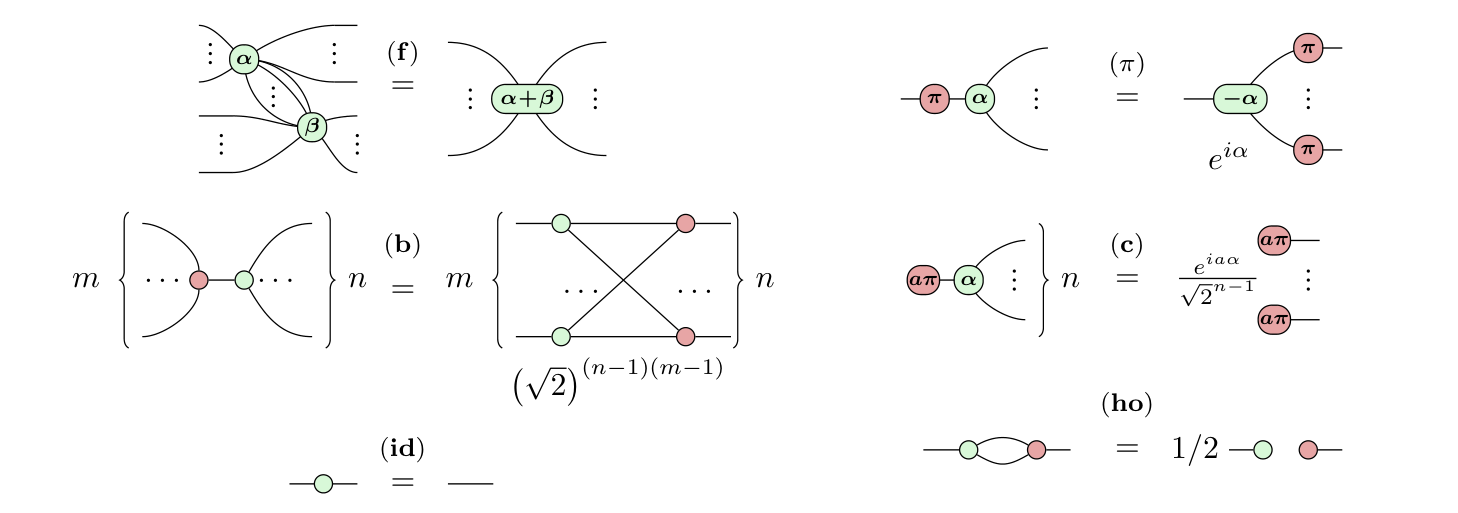
\includegraphics[width=\textwidth]{figures/zx_rewrite_rules_p1.png}
\end{figure}    
\end{frame}

\begin{frame}
    \begin{figure}
        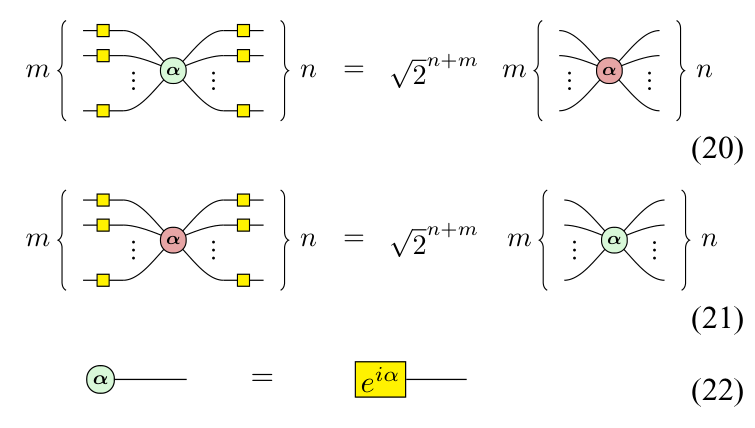
\includegraphics[width=\textwidth]{figures/zx_rewrite_rules_p2.png}
    \end{figure}
\end{frame}

\begin{frame}
    \begin{figure}
        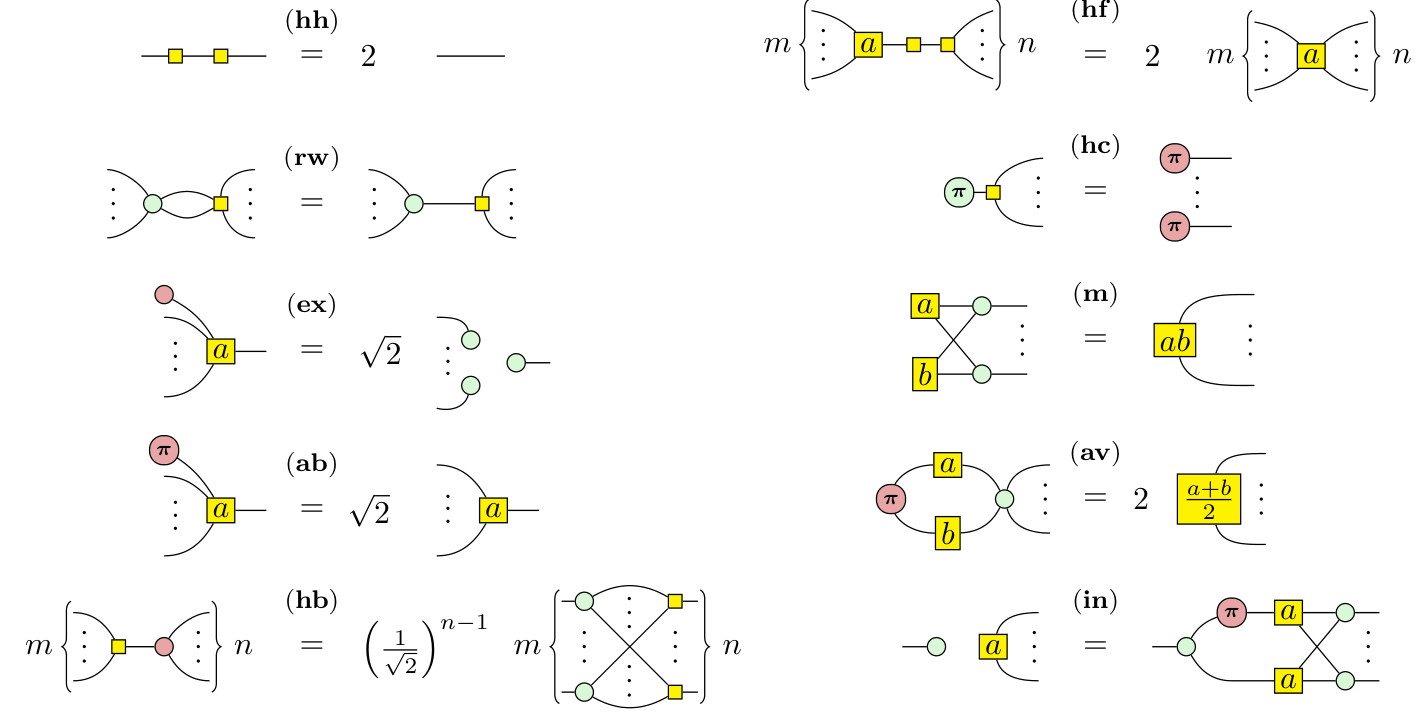
\includegraphics[width=\textwidth]{figures/zx_rewrite_rules_p3.png}
    \end{figure}
\end{frame}

\begin{frame}{Constructor of projector of higher spin}
    \begin{itemize}
        \item To represent spins $N/2$ sites, we stack $N$ spin-1/2 and project onto the symmetric subspace\footnote{Recall the highest spin subspace of N spin-1/2 is all the states that is symemtric under permutation of spin indices}
        \item This is done by the symmetrizing projector
        \begin{align*}
            P = \frac{1}{n!}\sum_{\sigma \in S_N} U_\sigma
        \end{align*}
        where $U_\sigma\ket{x_1 x_2\cdots} = \ket{x_{\sigma(1)}x_{\sigma(2)} \cdots}$
    \end{itemize}
\end{frame}

\begin{frame}
    \begin{itemize}
        \item Basically we want a coherent superposition of swap wires
        \item This is done by CSWAP which maps $\ket{0xy}\mapsto\ket{0xy}$ and $\ket{1xy}\mapsto\ket{1yx}$.
    \end{itemize}
    \begin{figure}
        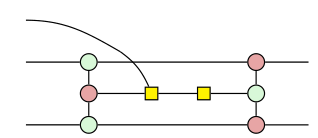
\includegraphics[width=.6\textwidth]{figures/cswap_two_qbit.png}
    \end{figure}
    \begin{itemize}
        \item Higher projectors can be constructed inductively by swapping additional qubit with all other qubits\footnote{There are some subtleties as to how to make sure only at most one CSWAP is fired each time. Details are presented in Appendix C of the paper.}
    \end{itemize}
    
\end{frame}


\begin{frame}{Higher spin representation of SU(2)}
    \begin{itemize}
        \item One way to represent arbitary spins is to stack $N$ spin-1/2 
        $$\overbrace{\mathbf{2} \otimes  \mathbf{2} \cdots \otimes \mathbf{2}}^{N \text{ copies}}$$
        \item The representation of $\mathfrak{su}(2)$ in this space is basically given by
        \begin{align*}
            \hat S_z = \sum_{i=1}^N \hat S_z^{(i)}\quad\quad 
            \hat S_\pm = \sum_{i=1}^{N}\hat S_x^{(i)}\pm i \hat S_y^{(i)}
        \end{align*}
    \end{itemize}
\end{frame}

\begin{frame}
    \begin{itemize}
        \item To construct a spin-N/2 subspace, we take the highest state $\ket{\uparrow \cdots \uparrow}$ and apply $\hat S_{-}$ repeatedly
        \item The highest state is obviously symmetric under permutation of spin label
        \vspace{.5cm}
        \item For any state obtained by applying $\hat S_{-}$, we note that 
        \begin{align*}
            \text{Perm}(\hat S_{-}\Ket{\psi},\sigma) = \text{Perm}(\hat S_{-}, \sigma) \text{Perm}(\ket{\psi},\sigma)
        \end{align*}
        where $\sigma \in S_N$ is a permutation of spin index 
        \item Since both $\hat S_{-}$ and $\ket{\psi}$ are totally symmetric, the state $\hat S_- \ket{\psi}$ must also be a totally symmetric state
        \vspace{.5cm}
        \item Therefore, the subspace spanned by totally symmetric states is the highest spin subspace.
    \end{itemize}
\end{frame}

\begin{frame}{Positive operator valued measure (POVM)}
    \begin{itemize}
        \item Let $\{\mathcal O_i\}$ be a set of positive semi-definite operators. The set of operator is said to form a positive operator value value measure (POVM) if they satisfy the completeness relations
        \begin{align*}
            \sum_i \mathcal O_i = I
        \end{align*}
        \item Since it is always possible to write $\mathcal O_i$ in terms of Kraus operators $E_i^\dagger E_i$, we can also express our relations in terms of Kraus operators
        \begin{align*}
            \sum_i  E_i^\dagger E_i = I
        \end{align*}
        \item $E_i$ are not unique because $E_i \mapsto U E_i$ where $U$ is unitary gives you another set of valid Kraus operators 
    \end{itemize}
\end{frame}

\begin{frame}
    \begin{itemize}
        \item The post-measurement state is not uniquely determined by $\mathcal O_i$
        \item However, given $E_i$, the post-measurement state is given by 
        \begin{align*}
            \ket{\psi} \mapsto \frac{E_i \ket{\psi}}{\braket{\psi|E_i^\dagger E_i|\psi}}
        \end{align*}
        \item Note that the post-measurement state is not uniquely defined by $\mathcal O_i$ as $E_i$ is undetermined up to a unitary $U$
        \item This agree with the notion that we need to supply in addition to $\mathcal O_i$ the exact form of $E_i$ to uniquely determine the post-meausrement state
    \end{itemize}
\end{frame}

\begin{frame}{Graph states}
    \begin{itemize}
        \item A simple graph $G=(V,E)$ consist of a set of vertices $V$ and a set of edges $E\subseteq \{\{x,y\} \in V\times V, x\neq y\}$
        \item Let $G$ be a graph, and $\ket{G}_0 = \ket{+}^{\otimes}$ be the empty graph state. The graph state $\ket{G}$ is defined as
        \begin{align*}
            \ket{G} = \prod_{(i,j) \in E} \mathcal U_{ij} \ket{G_0}
        \end{align*} 
        where $\mathcal U_{ij} =\text{CZ}(i,j)$ with $i,j \in V$  
        \item Equivalently, graph states can be understood using the stabilizer formalism
    \end{itemize}
\end{frame}

\begin{frame}
    \begin{itemize}
        \item A \textit{cluster state} is a graph state where the underlying graph is a lattice
        \item Any 2D cluster state is a universal resource for measurement-based quantum computation
        \item 
    \end{itemize}
\end{frame}

\begin{frame}
    \begin{itemize}
        \item The spin operator (with $\hbar$ stripped) for spin-1 systems are
        \begin{align*}
            S_x = \begin{pmatrix}
                0 & \frac{\sqrt{2}}{2} & 0 \\
                \frac{\sqrt{2}}{2} & 0 & \frac{\sqrt{2}}{2}\\
                0 & \frac{\sqrt{2}}{2} & 0
            \end{pmatrix}\quad S_y = \begin{pmatrix}
                0 & -i\frac{\sqrt{2}}{2} & 0 \\
                i\frac{\sqrt{2}}{2} & 0 & -i\frac{\sqrt{2}}{2}\\
                0 & i\frac{\sqrt{2}}{2} & 0
            \end{pmatrix} \quad S_z = \begin{pmatrix}
                1 & 0 & 0\\
                0 & 0 & 0\\
                0 & 0 & 1 
            \end{pmatrix}
        \end{align*}\vspace{1mm}
        \item Therefore the rotation operator of the group $\mathbb Z_2 \times \mathbb Z_2$ is represented as 
        \begin{align*}
            U_x(\pi) = \begin{pmatrix}
                0 & 0 & -1 \\
                0 & -1 & 0\\
                -1 & 0 & 0
            \end{pmatrix}\quad U_y(\pi) = \begin{pmatrix}
                0 & 0 & 1 \\
                0 & -1 &  0\\
                1 & 0 & 0
            \end{pmatrix}\quad U_z(\pi) =\begin{pmatrix}
                -1 & 0 & 0\\
                0 & 1 & 0\\
                0 & 0 & -1 
            \end{pmatrix}
        \end{align*}
        \item Note that these are the matrix representation in the spin-1 z basis
    \end{itemize}
\end{frame}

\begin{frame}
    \begin{itemize}
        \item Therefore, if we apply these transformations individually to each site, we have \begin{align*}
            A^{\sigma}_i \mapsto \sum_{\sigma=0,\pm 1}U^{\sigma'}_{\sigma} A_i^{\sigma}
        \end{align*}
        where $\sigma$ denote the $\sigma$-th component of the spin-1 spinor and $i$ is the site index.
        \item In particular 
    \end{itemize}
\end{frame}



%------------------------------------------------
% Refenrenced
\begin{frame}{References}
    % Beamer does not support BibTeX so references must be inserted manually as below
    \footnotesize{
        \begin{thebibliography}{99}

            \bibitem[van de Wetering,2020]{zx_for_working_qcs} John van de Wetering (2020)
            \newblock ZX-calculus for the working quantum computer scientist
            \newblock \emph{arXiv preprint arXiv:2012.13966}
            
            \bibitem[Hatsugai, 2006]{hatsugai2006quantized} Yasuhiro Hatsugai (2006)
            \newblock Quantized Berry phases as a local order parameter of a quantum liquid
            \newblock \emph{Journal of the Physical Society of Japan}, 75(12), 123601

            \bibitem[Wei et al., 2011]{wei2011_aklt_honeycomb} Tzu-Chieh Wei, Ian Affleck, and Robert Raussendorf (2011)
            \newblock Affleck-Kennedy-Lieb-Tasaki State on a Honeycomb Lattice is a Universal Quantum Computational Resource
            \newblock \emph{Phys. Rev. Lett.}, 106(7), 070501 DOI: 10.1103/PhysRevLett.106.070501
            \newblock URL: \url{https://link.aps.org/doi/10.1103/PhysRevLett.106.070501}
        \end{thebibliography}
    }
\end{frame}

%----------------------------------------------------------------------------------------
% Final PAGE
% Set the text that is showed on the final slide
\finalpagetext{Thank you for your attention}
%----------------------------------------------------------------------------------------
\makefinalpage
%----------------------------------------------------------------------------------------
\end{document}